%! Author = Joel Vontobel
%! Date = \today


\documentclass[11pt, a4paper]{report}

% Listings
\usepackage{listings}

\lstset{
    literate={ö}{{\"o}}1
        {ä}{{\"a}}1
        {ü}{{\"u}}1
}

\lstset{language=Java,
    basicstyle=\ttfamily,
    keywordstyle=\color{javapurple}\bfseries,
    stringstyle=\color{javared},
    commentstyle=\color{javagreen},
    morecomment=[s][\color{javadocblue}]{/**}{*/},
    numbers=left,
    numberstyle=\tiny\color{black},
    stepnumber=2,
    numbersep=10pt,
    tabsize=4,
    showspaces=false,
    showstringspaces=false}

% Packages
\usepackage[margin=1.4in]{geometry}
\usepackage[T1]{fontenc}
\usepackage[utf8]{inputenc}
\usepackage[ngerman]{babel}
\usepackage{hyperref}
\usepackage{verbatim}
\usepackage{graphicx}
\usepackage{float}
\usepackage{pdfpages}
\usepackage[
    singlelinecheck=false
]{caption}
\usepackage[raggedright]{titlesec}
\usepackage[nottoc]{tocbibind}
\usepackage{longtable}
\usepackage{tocloft}
\usepackage{fancyhdr}
\usepackage{lastpage}
\usepackage{pifont}
\usepackage{amsmath}

\usepackage[automake]{glossaries-extra}
\usepackage{wasysym}
\usepackage{textcomp}
\usepackage{color}



\titleformat{\chapter}{\normalfont\bfseries\LARGE\raggedright}{\thechapter}{1ex}{}
\titlespacing*{\chapter}{0pt}{30pt}{30pt}
\setcounter{secnumdepth}{3}
\setcounter{tocdepth}{3}
\setlength{\cftsecnumwidth}{2.8em}
\renewcommand\labelitemi{$-$}
\renewcommand\labelitemii{$-$}
\renewcommand\labelitemiii{$-$}
\renewcommand{\headrulewidth}{0pt}

\usepackage[
    backend=biber,
    citestyle=authoryear,
    style=authoryear,
]{biblatex}
\addbibresource{global/quellen.bib}

\usepackage[toc]{glossaries}
\makeglossaries
\loadglsentries{global/glossar_eintraege}

\pagestyle{fancy}
\fancyhf{}
\renewcommand{\headrulewidth}{0pt}
%TODO Platzhalter ersetzen
\lfoot{\fontsize{10}{15} \selectfont Joel Vontobel}
\cfoot{\fontsize{10}{15} \selectfont \today}
\rfoot{\fontsize{10}{15} \selectfont \thepage~von~\pageref*{LastPage}}
\fancypagestyle{plain}{}

\newcommand{\oksymbol}{{\color{green}\ding{51}}}
\newcommand{\errorsymbol}{{\color{red}\ding{55}}}

\makeatletter
\def\blx@citation#1#2{\blx@citation@entry{#1}{#2}}
\makeatother
\renewcommand{\arraystretch}{1.5}
% Document
\begin{document}

    \begin{titlepage}

    \begin{figure}
        \begin{center}
            
\includegraphics[width=0.6\textwidth]{ressourcen/ergon_logo_gross}
            \captionsetup{textformat=empty, labelformat=empty}
            \caption[Logo der Ergon Informatik AG~\parencite{ergonlogo}]{Logo der Ergon Informatik AG}\label{fig:ergon-logo-gross}
        \end{center}
    \end{figure}
    \begin{center}
        \vspace*{2cm}
        \Huge
        \textbf{Probe-IPA}

        \vspace{0.5cm}
        \Large
        %TODO Platzhalter ersetzen 
        Eingehende Message-Queue-Nachrichten im Web-UI

        \vfill

        \Large
        %TODO Platzhalter ersetzen
        Probe-IPA von Joel Vontobel

        \vspace*{3cm}

        \large
        Ergon Informatik AG\\
        \today\\

    \end{center}
\end{titlepage}

    \renewcommand*\contentsname{Inhalt}
\tableofcontents
    \part{Umfeld und Ablauf}\label{part:1}

    \chapter{Aufgabenstellung}\label{ch:aufgabenstellung}
In diesem Kapitel ist die Aufgabenstellung der Probe-IPA aufgeführt. Die Inhalte wurden zu einem grossen Teil von der originalen Aufgabenstellung übernommen und Angepasst.

\section{Ausgangslage}\label{sec:ausgangslage}
Die Firma \gls{Ergon Informatik AG} entwickelt sein einigen Jahren eine Transaktions-Authorisierungs-Lösung für einige Banken in der Schweiz. Dieses Projekt heisst \gls{CardX} und wird durch ein 12 zwölfköpfiges Team umgesetzt. In diesem Projekt ist der Lernende seit Januar 2024 tätig und kennt sich deshalb schon ein bisschen aus.

Das Projekt kommuniziert mit verschiedenen bankspeziefischen IT-Systemen wie zum Beispiel dem Kernbankensystem oder Service-Büros über Message-Queues. Diese Message-Queues werden in der Datenbank-Tabelle MQ\_TABLE (eingehende Nachrichten) und MQ\_OUT (ausgehende Nachrichten) zwischengespeichert. Falls man diese Message-Queues anschauen oder bearbeiten möchte, muss man dies in der Datenbank machen. Weil das ziemlich umständlich ist, besteht die Aufgabe des Lernenden jetzt daraus diese Message-Queues in einem \gls{Web-GUI} darzustellen und sinnvolle Interaktionen mit diesen Daten anzubieten.

\section{Detaillierte Aufgabenstellung}\label{sec:detaillierte-aufgabenstellung}

\paragraph{Minimalanforderungen}
Das Ziel dieser Aufgabe ist es, den Inhalt der Tabelle MQ\_TABLE in diesem Web-GUI sichtbar zu machen und dem Nutzer sinnvolle Interaktionen mit diesen Daten anzubieten.

Es soll im Weg-GUI eine neue Seite erstellt werden mit dem Inhalt einer Tabelle, welche die Message-Queues abbilden soll. Die Tabelle soll eine Hand voll Spalten besitzen, sodass sie übersichtlicher ist. Die Seite soll stimmig in das \gls{UI} eingebaut werden. Im \gls{Backend} sollen die neuen Methoden mithilfe von Unit-Tests abgedeckt werden.

Zusätzlich kann der Lernende noch zwischen zwei Erweiterungen entscheiden, welche er implementieren möchte.

\paragraph{Erweiterung: Pagination}
Bei der ersten Erweiterungen ist das Ziel ein Paginator zur Tabelle hinzuzufügen. Eine Pagination ist wenn man eine Liste oder Tabelle auf ein paar Einträge limitiert und anschliessend weitere Einträge anzeigen kann mit einer Pfeiltaste. Dies hilft, das Laden der Seite zu verkürzen, da die Einträge, die nicht angezeigt werden, erst geladen werden, wenn sie auch wirklich gebraucht werden.

\paragraph{Erweiterung: Filter}
Die zweite Erweiterung ist ein Filtersystem. Die Seite soll nach dem Status, Inhalt der Nachricht und dem Datum gefiltert werden können. Die Filter-Werte sollen ausserdem in der URL Abgebildet werden, um das Teilen von gefilterten Ergebnissen zu vereinfachen oder den Filter als Lesezeichen abgelegen zu können.

\section{Mittel und Methoden}\label{sec:mittel-und-methoden}

\paragraph{Technologien}
\begin{itemize}
	\item SQL
    \item Java
    \item TypeScript
    \item HTML
    \item Angular
\end{itemize}

\paragraph{Tools}
\begin{itemize}
	\item IntelliJ (IDE)
    \item Docker
	\item Bitbucket
	\item Confluence
	\item Jira
	\item Postman
\end{itemize}

\section{Vorkenntnisse}\label{sec:vorkenntnisse}
Der Lernende hat bereits viele Arbeiten im Projekt CardX gemacht. Unter anderem im Backend und an CardX-spezifischen Tools. Die Codebasis hat der Lernende in den letzten 9 Monaten gut kennengelernt und findet sich gut zurecht. Der Lernende hat auch bereits die Tabelle TASK von der Datenbank in das Web-GUI gebracht, was eine ähnliche Aufgabe war wie die jetzige Aufgabenstellung.

Durch die früheren Projekte, wie ein Fussballtippspiel und eine Anmelde-Plattform für Bewerbende, konnte er bereits viel Erfahrung mit Java und Angular sammeln.

\section{Vorarbeiten}\label{sec:vorarbeiten}
Durch das bereits existierende Projekt und die vielen Arbeiten, die der Lernende bereits gemacht hat, musste er keine Vorarbeiten leisten.

\section{Neue Lerninhalte}\label{sec:neue-lerninhalte}
\begin{itemize}
    \item Pagination: 
    
    Mit Pagination hat der Lernende sich noch nie auseinandergesetzt. Er hat es schon oft auf anderen Seiten gesehen aber noch nie selbst implementiert.
    \item Filtersystem:
    
    Im Projekt WM-Tippspiel gab es ein Filtersystem, aber dieses hat der Lernende nicht selbst implementiert und ist so ein neuer Lerninhalt.
\end{itemize}

\section{Arbeiten in den letzten 6 Monaten}\label{sec:arbeiten-in-den-letzten-6-monaten}
In den letzten 6 Monaten hat der Lernende sich, wie oben schon genannt, mit dem Projekt CardX auseinandergesetzt und ist ein aktives Team Mitglied. Er hat viele verschiedene Arbeiten umgesetzt. Einige davon hier:
\begin{itemize}
    \item CheckDB Task:
    
    In dieser Aufgabe geht es darum, eine Aufgabe zu erstellen, welche periodisch oder manuell ausgeführt werden kann. Diese Aufgabe überprüft die Datenbankdefinition, ob immer noch alles fehlerfrei ist. Es werden Sequenzen, Indexe, Felder und mehr in eine Datei geschrieben, gespeichert und anschliessend mit der vorherigen Datei auf Veränderungen verglichen. Bei einer Veränderung schlägt die Aufgabe fehl und die Differenz wird in der Fehlermeldung angezeigt.
    \item ServiceLogMove und Zip:
    
    Mit der Aufgabe ServiceLogMerge werden Protokolle des Systems in Dateien geschrieben und gespeichert. Ein Teil dieser Dateien wird jetzt mithilfe der Aufgabe in bestimmte Verzeichnisse verschoben und komprimiert. Die Dateien werden nach Bank sortiert und anschliessend in ihn vorgesehenes Verzeichnis verschoben. Auch diese Aufgabe wird periodisch jeden Tag ausgeführt, um die Dateiablage übersichtlich zu halten.
    \item Tasks im Frontend anzeigen und bearbeiten:
    
    Diese Aufgabe zeigt alle Tasks im Frontend an und man kann sie dort auch bearbeiten. Das Ziel von dieser Aufgabe war gleich wie die Mindestanforderungen von der Aufgabenstellung.
    \begin{figure}[H]
    	\begin{center}
    		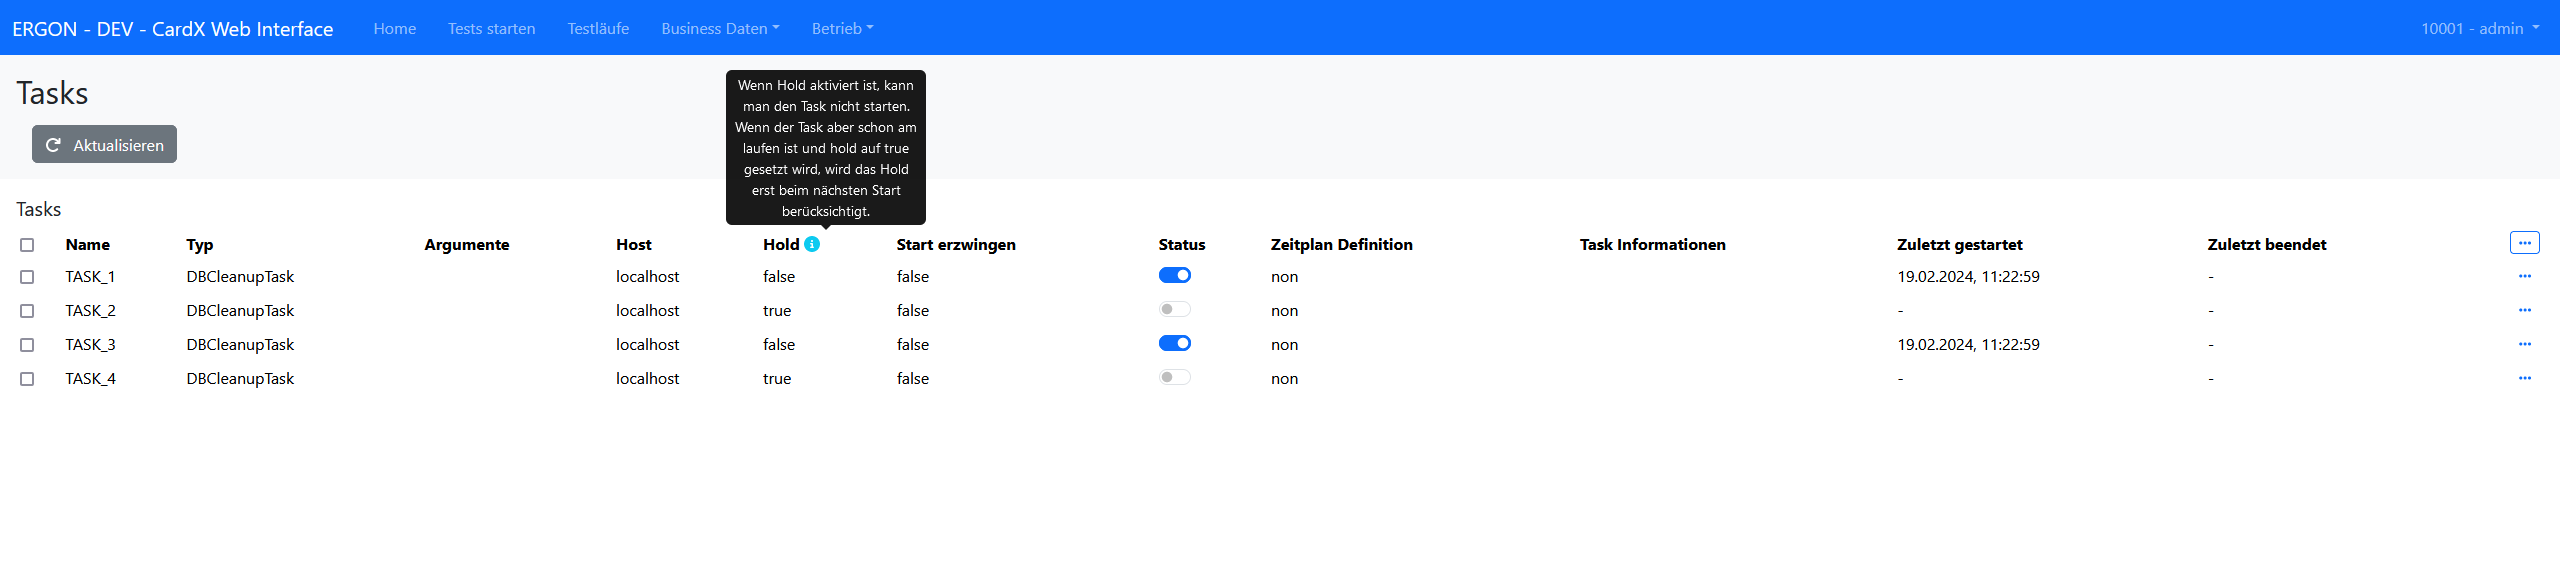
\includegraphics[width=1\textwidth]{ressourcen/show-and-edit-tasks}
    		\caption[Anzeigen und bearbeiten der Tasks]{Anzeigen und bearbeiten der Tasks}\label{fig:show-and-edit-tasks}
    	\end{center}
    \end{figure}
\end{itemize}

    \chapter{Projektaufbauorganisation}\label{ch:projektaufbauorganisation}
In der folgenden Tabelle sind die an der Probe-IPA beteiligten Personen und ihre jeweiligen Aufgaben aufgeführt.

\renewcommand{\arraystretch}{1.5}
\begin{longtable}{|p{.30\textwidth}|p{.30\textwidth}|p{.40\textwidth}|}
    \hline
    \textbf{Person} & \textbf{Rolle} & \textbf{Aufgabe/Verantwortung} \\
    \hline
    %TODO Platzhalter ersetzen
    \hypertarget{k}{Joel Vontobel} & Kandidat (K) & Umsetzen der Facharbeit \\
    \hline
    %TODO Platzhalter ersetzen
    \hypertarget{vf}{Loris Diana und Dominic Monzón} & Verantwortliche Fachkraft (VF) & Facharbeit begleiten, technische Fragen beantworten, Bewertung der Facharbeit \\
    \hline
    %TODO Platzhalter ersetzen
    \hypertarget{hex}{Bernd Lienberger} & Hauptexperte (HEX) & IPA bezogene Fragen beantworten, Entscheiden bei auftretenden Problemen, Besuchstermine festlegen, Fachgespräch leiten, Bewertung der Facharbeit \\
    \hline
    %TODO Platzhalter ersetzen
    \hypertarget{nex}{} & Nebenexperte (NEX) & Notizen erstellen zu Präsentation und zum Fachgespräch, Bewertung der Facharbeit \\
    \hline
\end{longtable}
\renewcommand{\arraystretch}{1}

    \chapter{Arbeitsumgebung}\label{ch:arbeitsumgebung}
In diesem Kapitel ist beschrieben, wie die Arbeitsumgebung des Lernenden während der Probe-IPA aussah.


\section{Arbeitsplatz}\label{sec:arbeitsplatz}
\subsection{Office Arbeitsplatz}\label{subsec:office-arbeitsplatz}
Die Probe-IPA wird am gewohnten Arbeitsplatz im Fünferbüro des Lernenden durchgeführt. Als Arbeitsgerät wird ein Notebook verwendet, welches mithilfe einer Dockingstation das Gerät mit zwei Monitoren und dem Firmennetzwerk verbindet. Der Stuhl und Tisch sind höhenverstellbar, und der Lernende kann dadurch in verschiedenen Sitzpositionen oder stehend arbeiten.

\begin{figure}[H]
    \begin{center}
        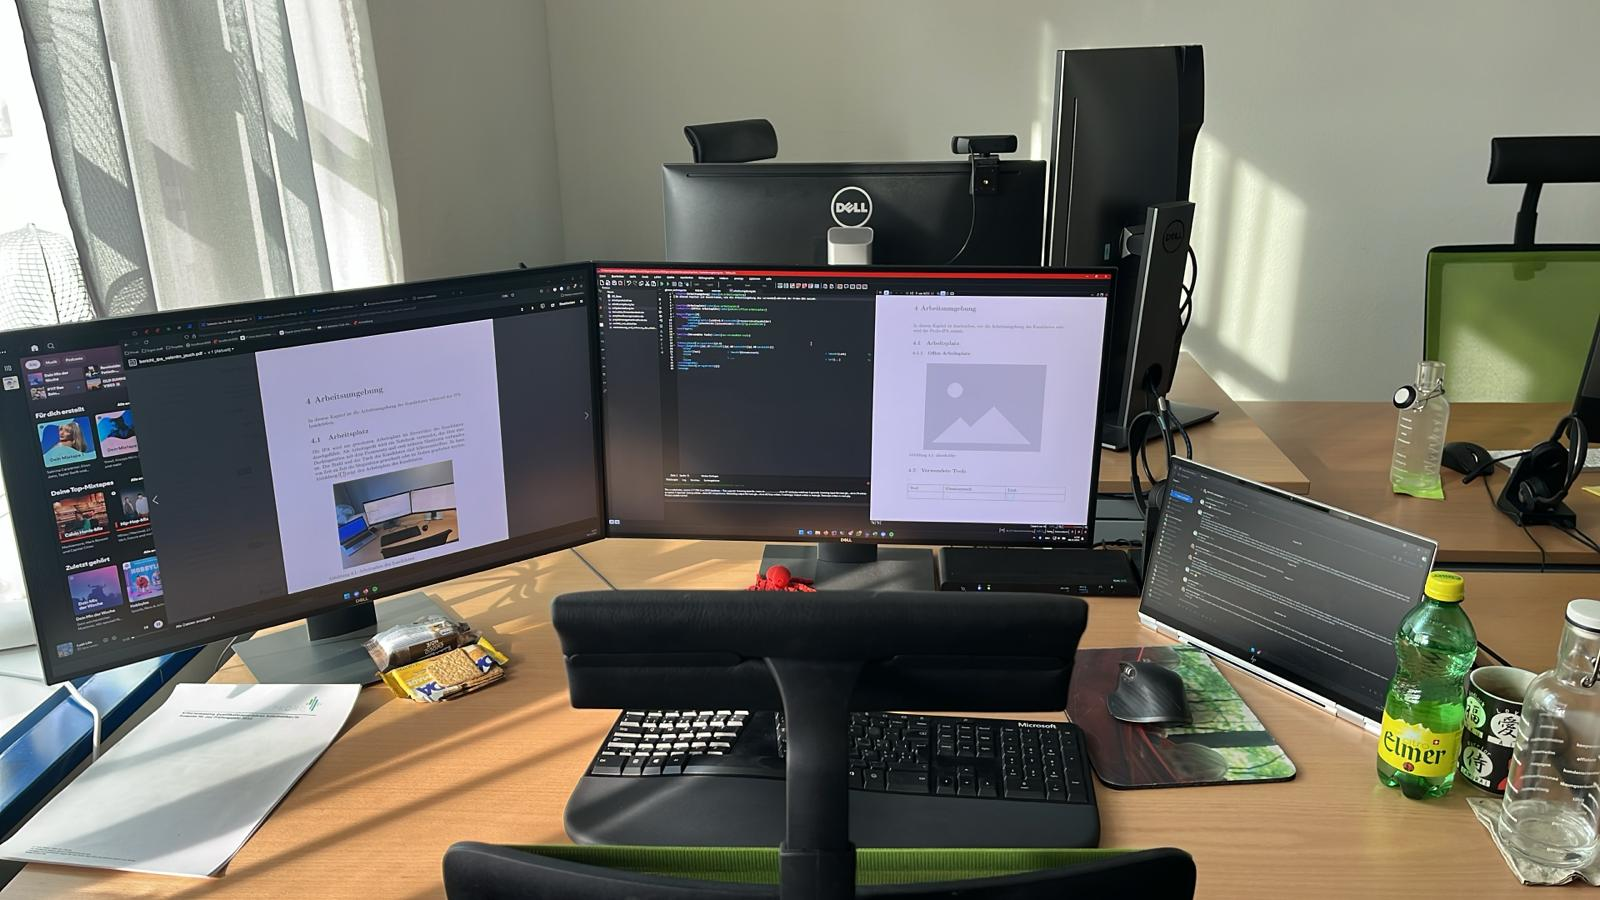
\includegraphics[width=0.8\textwidth]{ressourcen/Arbeitsplatz-Joel-Vontobel}
        \caption[Arbeitsplatz des Lernenden]{Arbeitsplatz des Lernenden}\label{fig:Arbeitsplatz-Joel-Vontobel}
    \end{center}
\end{figure}

\newpage
\section{Verwendete Tools}\label{sec:verwendete-tools}
Die folgende Tabelle zeigt auf, welche Tools für die Umsetzung der Probe-IPA eingesetzt wurden.

\renewcommand{\arraystretch}{1.5}
\begin{longtable}{|p{.22\textwidth}|p{.40\textwidth}|p{.38\textwidth}|}
    \hline
    \textbf{Tool}                    & \textbf{Einsatzzweck}                              & \textbf{Link}                                                             \\ \hline
    IntelliJ                         & Entwicklungsumgebung für die Programmierung        & \url{https://www.jetbrains.com/de-de/idea/}                               \\ \hline
    Docker                           & Ausführen der Programme                            & \url{https://www.docker.com/}                                             \\ \hline
    Git                              & Versionierung vom Quellcode                        & \url{https://git-scm.com/}                                                \\ \hline
    Postman                          & Ausführen von HTTP-Requests (Testen vom Bankend)   & \url{https://www.postman.com/}                                            \\ \hline
    Bitbucket                        & Speicherung der Quellcodes                         & \url{https://bitbucket.org/product/}                                      \\ \hline
    Confluence                       & Probe-IPA Kriterien                                & \url{https://www.atlassian.com/de/software/confluence}                    \\ \hline
    Jira                             & Aufgabenstellung                                   & \url{https://www.atlassian.com/de/software/jira}                          \\ \hline
    Draw.io                          & Erstellen von Diagrammen und Abbildungen           & \url{https://www.drawio.com/}                                             \\ \hline
    TexStudio                        & Dokumentationstool                                 & \url{https://www.texstudio.org/}                                          \\ \hline
    LaTeX                            & Ein Dokumentenvorbereitungssystem                  & \url{https://www.latex-project.org/}                                      \\ \hline
    Mattermost                       & Text basiertes Kommunikationsmittel                & \url{https://mattermost.com/}                                             \\ \hline
    Microsoft Teams                  & Video basiertes Kommunikationiesmittel             & \url{https://www.microsoft.com/de-ch/microsoft-teams/group-chat-software} \\ \hline
    Microsoft Excel                  & Erstellung und Bearbeitung des Zeitplans           & \url{https://www.microsoft.com/de-ch/microsoft-365/excel?market=ch}       \\ \hline
\end{longtable}
\renewcommand{\arraystretch}{1}
\newpage
    \chapter{Versionierung und Sicherung der Arbeitsergebnisse}\label{ch:versionierung-und-sicherung-der-arbeitsergebnisse}
In diesem Kapitel wird beschrieben, wie der Lernende sicherstellt, dass die erarbeiteten Ergebnisse während der Probe-IPA sicher gespeichert und jederzeit wieder aufrufbar sind. Die Versionierung soll es ermöglichen, frühere erstellte Versionen der Daten jederzeit wiederherstellen zu können. Die Massnahmen werden hier vom Lernenden aufgeführt.

\section{Verwendung von Git zu Versionierung}
Für die Versionierung von der Probe-IPA wird Git verwendet. Git ist ein Versionierungstool und wird verwendet, um Quellcode zu versionieren und zu beschriften. In der Schule so wie auch in der Firma wurde Git bereits in diversen Projekten verwendet, um den Quellcode übersichtlich zu versionieren und in der Cloud zu sichern. Mit Git kann man sogenannte «Commits» machen, um einen kleinen Teil der Änderungen zu speichern und zu beschriften. Diese Änderungen kann man jederzeit aufrufen oder wieder rückgängig machen, um eine bestimmte Version genauer zu analysieren. Durch diese Commits ist der Quellcode für eine andere Person verständlicher und einfacher zu lesen.

\section{Quellcode}
Der Quellcode der eingehenden Message-Queue-Nachrichten im Web-GUI wird mit Git verwaltet und ist in einem Repository auf Bitbucket gespeichert. In Abbildung 5.1 ist die Git Commit History des Quellcodes ersichtlich.

\begin{figure}[H]
	\begin{center}
		
\includegraphics[width=0.8\textwidth]{ressourcen/placeholder}
		\caption[Git Commit History des Quellcodes]{Git Commit History des Quellcodes}\label{fig:Git-Commit-History-des-Quellcodes}
	\end{center}
\end{figure}

\section{Probe-IPA Dokumentation}
Die Probe-IPA-Dokumentation wird mithilfe von \LaTeX geschrieben, wodurch eine Versionierung mit Git auch möglich wird. Die \LaTeX- und alle anderen benötigten Dateien werden auf ein privates Repository in der Cloud geladen. In Abbildung 5.2 ist die Git Commit History der Probe-IPA-Dokumentation ersichtlich.

\begin{figure}[H]
	\begin{center}
		
\includegraphics[width=0.8\textwidth]{ressourcen/placeholder}
		\caption[Git Commit History der Dokumentation]{Git Commit History der Dokumentation}\label{fig:Git-Commit-History-der-Dokumentation}
	\end{center}
\end{figure}
    \chapter{Projektmanagementmethode}\label{ch:projektmanagementmethode}
In diesem Kapitel ist die Projektmanagement-Methode «IPERKA» beschrieben, die während der Probe-IPA verwendet wird. Es werden die Gründe für diese Projektmanagement-Methode aufgeführt und eine alternative Methode mit Gründen, warum sie nicht verwendet wurde.

\section{IPERKA}\label{sec:METHODE}
Als Projektmanagement-Methode während der Probe-IPA wird IPERKA verendet. IPERKA ist eine Vorgehensmethode, die sich gut für Projekte mit überschaubarem Umfang und klar definierte Ziele eignet. Die Methode wirde bereits im ersten Lehrjahr in der Schule behandelt und ist durch das bereits bekannt. Der Name «IPERKA» setzt sich aus den Anfangsbuchstaben der sechs verschiedenen Schritten zusammen, nach denen vorgegangen wird:

\paragraph{I} nformieren: Den Auftrag verstehen, eine Vorstellung der Lösung erhalten, fehlende Informationen einholen, ordnen und bewerten
\paragraph{P} lanen: Nötige Arbeitsschritte definieren, einen Zeitplan erstellen, Methoden und Arbeitsmittel definieren
\paragraph{E} ntscheiden: Verschiedene Lösungsvarianten vergleichen, ausschlaggebende Kriterien definieren, eine Lösungsvariante auswählen
\paragraph{R} ealisieren: Arbeit umsetzen, Arbeitsschritte und Ergebnisse dokumentieren, auftrettende Probleme behandeln
\paragraph{K} ontrollieren: Arbeit testen, Resultate mit den Anforderungen vergleichen, Soll-Ist-Vergleich des Zeitplans, Dokumentation nochmals durchlesen
\paragraph{A} uswerten: Rückblick auf das Vorgehen, Arbeitsschritte beurteilen, Selbsteinschätzung vornehmen, mögliche Optimierungen für weitere Projekte definieren

\pagebreak
Die Aufteilung der Arbeit in die genannten Schritte unterstützt dabei, die Aufgaben sinnvoll zu strukturieren und systematisch vorzugehen. Ausserdem hilft die bewusste Steuerung des Arbeitsprozesses, die persönlichen Kompetenzen weiterzuentwickeln (vgl. ICT Berufsbildung Bern 2024\parencite{ict}). Die klare Trennung der Schritte stellt sicher, dass der Umfang und die erwarteten Ergebnisse der Aufgabe sich im Verlauf der Arbeit nicht mehr stark ändern, da IPERKA grundsätzlich kein «Rückwärtsgehen» in den Phasen, wie dies aus iterativen Modellen bekannt ist, vorsieht. Ausserdem stellt sie sicher, dass die Realisierung nicht zu schnell in Angriff genommen wird.

\section{Alternative Methode}\label{sec:alternative-methode}
Neben IPERKA wurde noch eine andere Vorgehensmethode angeschaut. Diese ist folgend, jeweils mit einer Begründung, wieso IPERKA der Methode vorgezogen wurde, kurz beschrieben.

\paragraph{Scrum} ist eine bekannte agile Vorgehensmehtode, die heutzutage in der Softwareentwicklung weit verbreitet ist. Die Methode legt den Fokus mehr auf Punkte wie laufende Software, gute Zusammenarbeit, oder flexibles Reagieren auf Veränderungen, ansttt einem strikten Plan zu folgen. Scrum sieht einen iterativen Prozess vor, der laufend optimiert werden soll, und definiert verschiedene Rollen, die jeweils ihre Aufgabe in diesem Scrum-Prozess haben. Ein «agiles» Vorgehen ist in der Softwareentwicklung grundsätzlich sinnvoll, da oft nicht von Beginn her klar ist, wie das Resultat schlussendlich aussehen soll. Da die Probe-IPA schlussendlich aber eine Prüfung ist, sind die Vorgaben und erwarteten Resultate relativ klar. Auch der Umfang der Probe-IPA und das Enddatum sind von Beginn an bekannt und verändern sich nicht während der Arbeit. Ausserdem wird die Aufgabe von nur einer Person bearbeitet, wofür die Abläufe von Scrum nicht optimal geeignet sind. Aus diesen Gründen wird IPERKA gegenüber Scrum vom Lernenden bevorzugt.

    \chapter{Zeitplan}\label{ch:zeitplan}
Basierend auf den definierten Arbeitspaketen wird ein Zeitplan erstellt, der als Richtwert für die Zehn Tage dient. Die Felder sind in 2-Stunden-Blöcken aufgeteilt. Bei der Arbeit selbst kann aber auf eine Stunde gerundet werden. Aus diesem Grund können auch zwei verschiedene Arbeitspakete auf einer Linie sein. Links am Rand sind die verschiedenen Arbeitspakete beschriftet und haben rechts davon den geschätzten Zeitaufwand (blaue Kästchen), tatsächlichen Zeitaufwand (gelbe Kästchen) und die Differenz.

\begin{figure}[H]
	\begin{center}
		
\includegraphics[width=0.8\textwidth]{ressourcen/placeholder}
		\caption[Zeitplan]{Zeitplan}\label{fig:zeitplan}
	\end{center}
\end{figure}

    \chapter{Arbeitsprotokoll}\label{ch:arbeitsprotokoll}
\renewcommand{\arraystretch}{1.5}

\begin{longtable}{p{.22\textwidth}|p{.78\textwidth}}
	\hline
	\textbf{Datum}                       & 06.11.2024            \\
	\hline
	\textbf{Bearbeitete Arbeitspakete}   & 7.1, 7.2, 7.3, 7.4                  \\
	\hline
	\textbf{Arbeitszeit}                 & 8h                                    \\
	\hline
	\textbf{Überzeit}                    & 0h                                    \\
	\hline
	\textbf{Vergleich mit dem Zeitplan}  & Zeitplan noch nicht fertig \\
	\hline
	\textbf{Erfolge und Probleme} & Durch die Vorlage des Dokuments und \LaTeX konnte ich direkt mit dem ersten Teil der Dokumentation beginnen, was mir viel Zeit erspart hat. Ich habe heute mein Ziel, den ersten Teil grösstenteils abzuschliessen, erreicht und hatte keine grösseren Probleme, die aufgetreten sind.
	\\
	\hline
	\textbf{Tagesreflexion} & Ich bin heute gut in die Probe-IPA gestartet. Anfangs war ich ein wenig überfordert und wusste nicht, wo ich anfangen sollte. Nach der ersten Stunde hat sich das aber wieder gelegt und ich konnte konzentriert an meinem Ziel arbeiten.
	\\
	\hline
	\textbf{In Anspruch genommene Hilfe} & Keine                              \\
	\hline
\end{longtable}\label{tab:arbeitsprotokoll-06.11.2024}
\newpage

\begin{longtable}{p{.22\textwidth}|p{.78\textwidth}}
	\hline
	\textbf{Datum}                       & 07.11.2024            \\
	\hline
	\textbf{Bearbeitete Arbeitspakete}   & 1.1, 1.2, 2.1, 2.2                  \\
	\hline
	\textbf{Arbeitszeit}                 & 8h                                    \\
	\hline
	\textbf{Überzeit}                    & 0h                                    \\
	\hline
	\textbf{Vergleich mit dem Zeitplan}  & Ich konnte alle geplanten Arbeiten von heute erledigen und hatte auch eine Stunde übrig. Ich habe also bereits mit der Aufgabe 2.3 angefangen. \\
	\hline
	\textbf{Erfolge und Probleme} & Heute konnte ich mit dem 2. Teil der Dokumentation anfangen. Die Phase Informieren konnte ich zeitgerecht abschliessen und habe bereits in der Phase Planen die Arbeitspakete und den Zeitplan fertiggestellt. Momentan habe ich mit der Aufgabe \ref{tab:planen-2.3} begonnen, die für morgen eingeplant ist.
	\\
	\hline
	\textbf{Tagesreflexion} & Ich konnte heute motiviert in den Tag starten, da ich gestern meine Tagesziele erreicht habe. Ich konnte mich nicht wirklich für \ref{tab:informieren-1.1} und \ref{tab:informieren-1.2} motivieren, wusste aber, dass ich mich danach mit den Arbeitspaketen und dem Zeitplan beschäftigen kann. Diese zwei Teile haben mir Spass gemacht, da ich mich danach am Zeitplan orientieren kann.
	\\
	\hline
	\textbf{In Anspruch genommene Hilfe} & Ich habe mich bei Loris Diana \ref{ch:projektaufbauorganisation} erkundigt, ob ich die Codequalität mit dem Tool, welches mein Projekt nutzt, überprüfen darf oder ich selbst diese Überprüfung machen muss.                                \\
	\hline
\end{longtable}\label{tab:arbeitsprotokoll-07.11.2024}
\newpage

\begin{longtable}{p{.22\textwidth}|p{.78\textwidth}}
	\hline
	\textbf{Datum}                       & 08.11.2024            \\
	\hline
	\textbf{Bearbeitete Arbeitspakete}   & 2.3, 2.4                  \\
	\hline
	\textbf{Arbeitszeit}                 & 8h                                    \\
	\hline
	\textbf{Überzeit}                    & 0h                                    \\
	\hline
	\textbf{Vergleich mit dem Zeitplan}  & Ich konnte alle geplanten Arbeitspakete machen oder anfangen.  \\
	\hline
	\textbf{Erfolge und Probleme} & Heute hatte ich Probleme mit der Konzentration. Sie ist schwungartig gekommen und wieder gegangen. Durch das habe ich ein wenig Zeit verloren und bin jetzt wieder im Zeitplan. Mein Ziel für heute war eigentlich, das Arbeitspaket 2.5 fertig zu haben, sodass ich nächste Woche mit dem Testkonzept starten kann. Ich habe es nicht ganz geschafft. Es fehlt aber nicht mehr viel.
	\\
	\hline
	\textbf{Tagesreflexion} & Wie bei «Erfolge und Probleme» schon erwähnt, fehlte mir heute ein wenig die Konzentration. Ich glaube, es könnte mit der VA zusammenhängen, da ich diese Woche noch daran gearbeitet habe und ich so mehrheitlich am Schreiben war. Ansonsten kann ich mich nicht beklagen, da ich immer noch ein kleines bisschen im Vorsprung zum Zeitplan bin.
	\\
	\hline
	\textbf{In Anspruch genommene Hilfe} & Ich habe mich heute bei Dominic Monzón \ref{ch:projektaufbauorganisation} erkundigt, ob für die Filterung alle MQ\_IN\_STATI gebraucht werden, weil im Quellcode die einen mit «// TODO huberdav: can be removed eventually» beschriftet sind.                                \\
	\hline
\end{longtable}\label{tab:arbeitsprotokoll-08.11.2024}
\newpage

\begin{longtable}{p{.22\textwidth}|p{.78\textwidth}}
	\hline
	\textbf{Datum}                       & 12.11.2024            \\
	\hline
	\textbf{Bearbeitete Arbeitspakete}   & 2.5                  \\
	\hline
	\textbf{Arbeitszeit}                 & 3.5h                                    \\
	\hline
	\textbf{Überzeit}                    & -0.5h                                    \\
	\hline
	\textbf{Vergleich mit dem Zeitplan}  & Momentan bin ich auf Kurs mit dem Zeitplan und habe keine Abweichungen. \\
	\hline
	\textbf{Erfolge und Probleme} & Alle Lösungskonzepte sind fertig und ich konnte mit den Testkonzepten anfangen.
	\\
	\hline
	\textbf{Tagesreflexion} & Heute kam ich gut voran und bin immer noch im Zeitplan. Der Vorsprung von letzter Woche ist heute jedoch nicht mehr vorhanden, aber ich bin nicht im Verzug. Heute war die Konzentration wieder hoch und ich hoffe, das bleibt auch für die bleibenden Tage noch weiter so.
	\\
	\hline
	\textbf{In Anspruch genommene Hilfe} & Ich habe mich bei Loris Diana \ref{ch:projektaufbauorganisation} erkundigt, ob ein Integration-Test für einen Endpoint eine Datenbank braucht, die läuft. Er hat mir erklärt, dass es eine braucht, aber auch eine In-Memory-Datenbank ausreicht.                              \\
	\hline
\end{longtable}\label{tab:arbeitsprotokoll-12.11.2024}
\newpage

\begin{longtable}{p{.22\textwidth}|p{.78\textwidth}}
	\hline
	\textbf{Datum}                       & 13.11.2024            \\
	\hline
	\textbf{Bearbeitete Arbeitspakete}   & 2.6, 3.1, 4.1                  \\
	\hline
	\textbf{Arbeitszeit}                 & 8.5h                                    \\
	\hline
	\textbf{Überzeit}                    & 0.5h                                    \\
	\hline
	\textbf{Vergleich mit dem Zeitplan}  & Durch die nicht verwendeten 3 Stunden von der Entscheidung wurde ich heute bei dem Punkt 4.1 zwei Stunden früher als geplant fertig. \\
	\hline
	\textbf{Erfolge und Probleme} & Heute konnte ich nach vielen Tagen Dokumentation schreiben, endlich mit dem Programmieren anfangen. Ich habe den Endpunkt bereits fertig und Dokumentiere diesen jetzt.
	\\
	\hline
	\textbf{Tagesreflexion} & Mit viel Motivation startete ich heute in den Tag, da ich wusste, dass ich endlich mit dem Programmieren anfangen kann. Ich habe das Textkonzept fertig geschrieben und konnte ziemlich schnell die Entscheidung abschliessen und habe so zwei Meilensteine in meiner Probe-IPA erreicht.
	\\
	\hline
	\textbf{In Anspruch genommene Hilfe} & Ich hatte Probleme mit einem Bean in Java, welches für den MqInService gebraucht wurde. Dieses wurde nicht gefunden und Dominic Monzón \ref{ch:projektaufbauorganisation} hat mir geholfen, dieses für den Service zu erstellen. Ausserdem konnte ich den Endpoint nicht ansprechen, da die Url fälschlicherweise falsch war und habe mir Hilfe von Micha Schena geholt (Ein Mitarbeiter im CardX-Team).                              \\
	\hline
\end{longtable}\label{tab:arbeitsprotokoll-13.11.2024}
\newpage

\begin{longtable}{p{.22\textwidth}|p{.78\textwidth}}
	\hline
	\textbf{Datum}                       & 14.11.2024            \\
	\hline
	\textbf{Bearbeitete Arbeitspakete}   & 4.2                  \\
	\hline
	\textbf{Arbeitszeit}                 & 8h                                    \\
	\hline
	\textbf{Überzeit}                    & 0h                                    \\
	\hline
	\textbf{Vergleich mit dem Zeitplan}  & Momentan bin ich synchron mit dem Zeitplan. \\
	\hline
	\textbf{Erfolge und Probleme} & Heute konnte ich die Mindestanforderungen abschliessen und mit der Erweiterung weiter machen.
	\\
	\hline
	\textbf{Tagesreflexion} & Ich konnte heute wieder mit viel Motivation in den Tag starten, da heute die Implementierung im Frontend bevor stand. Ich hatte länger als gedacht, da ich gestern einen Endpoint vergessen habe zu implementieren, welcher ich heute nacharbeiten musste.
	\\
	\hline
	\textbf{In Anspruch genommene Hilfe} & Loris Diana \ref{ch:projektaufbauorganisation} hat mir heute erklärt, wie die Generierung von den HTTP-Requests im Frontend genau funktioniert.                              \\
	\hline
\end{longtable}\label{tab:arbeitsprotokoll-14.11.2024}
\newpage

\begin{longtable}{p{.22\textwidth}|p{.78\textwidth}}
	\hline
	\textbf{Datum}                       & 15.11.2024            \\
	\hline
	\textbf{Bearbeitete Arbeitspakete}   & 4.3, 4.5                  \\
	\hline
	\textbf{Arbeitszeit}                 & 8h                                    \\
	\hline
	\textbf{Überzeit}                    & 0h                                    \\
	\hline
	\textbf{Vergleich mit dem Zeitplan}  & Da ich die Implementation von 4.4 \ref{tab:realisieren-4.4} pausiert habe, bin ich wieder synchron mit dem Zeitplan. \\
	\hline
	\textbf{Erfolge und Probleme} & Heute hatte ich viele Schwierigkeiten mit der Implementierung der Erweiterung im Frontend. Trotz des Beispiels von «Fehlgeschlagene Zahlung», schaffte ich es nicht, ein Filterergebnis im Frontend anzeigen zu lassen. Ich habe vieles ausprobiert und werde, falls noch Zeit ist, mit einem Fachverantwortlichen das Problem nochmals angehen.
	\\
	\hline
	\textbf{Tagesreflexion} & Ich hatte heute viel Motivation, um die Implementierung für den grössten Teil zu ermöglichen. Leider schwand diese Motivation ziemlich schnell während der Implementierung der Erweiterung im Frontend. Anfangs kam ich noch gut voran. Mit der Zeit wusste ich aber nicht, ob diese Implementierung funktionieren wird oder nicht. Da ich für beide Implementationen (das Backend und Frontend der Erweiterung) noch keine Dokumentation geschrieben habe, habe ich mich dazu entschieden, die Implementation zu pausieren und damit anzufangen, sodass ich nicht noch mehr in den Verzug komme.
	\\
	\hline
	\textbf{In Anspruch genommene Hilfe} & Dominic Moncón \ref{ch:projektaufbauorganisation} hat mir heute eine Frage bezüglich der Filterung beantwortet. Für die Filterung von Nachrichten konnte ich nicht auf die entsprechende Spalte zugreifen, und die Frage war, wie ich jetzt auf sie zugreifen kann. Bei anderen Feldern gibt es eine Variable, welche dies ermöglicht. Oberhalb der Felder steht aber, dass sie generiert wurden, und ich wusste nicht, ob ich sie direkt in dieser Klasse hinzufügen kann oder ob ich anderswo eine kleine Änderung unternehmen muss. Ich konnte schlussendlich einfach diese Variable hinzufügen.                           \\
	\hline
\end{longtable}\label{tab:arbeitsprotokoll-15.11.2024}
\newpage

\begin{longtable}{p{.22\textwidth}|p{.78\textwidth}}
	\hline
	\textbf{Datum}                       & 19.11.2024            \\
	\hline
	\textbf{Bearbeitete Arbeitspakete}   & 5.1 (angefangen)                  \\
	\hline
	\textbf{Arbeitszeit}                 & 3h                                    \\
	\hline
	\textbf{Überzeit}                    & -1h                                    \\
	\hline
	\textbf{Vergleich mit dem Zeitplan}  & Im Moment bin ich noch im Zeitplan. \\
	\hline
	\textbf{Erfolge und Probleme} & Heute konnte ich die Phase Realisieren abschliessen und mit der Implementierung der Tests anfangen. 
	\\
	\hline
	\textbf{Tagesreflexion} & Ich habe heute noch die Mock Implementation vom MqInService gemacht für das Akzeptanzkriterium. Dies ging ziemlich schnell und war nicht schwer zu implementieren. Ausserdem habe ich den ersten Test heute geschrieben, ohne grosse Probleme. Momentan kommen aber die hinzugefügten Daten in der Datenbank noch nicht im Test an. Dieses Problem werde ich aber morgen in Angriff nehmen. 
	\\
	\hline
	\textbf{In Anspruch genommene Hilfe} & -                              \\
	\hline
\end{longtable}\label{tab:arbeitsprotokoll-19.11.2024}
\newpage

\begin{longtable}{p{.22\textwidth}|p{.78\textwidth}}
	\hline
	\textbf{Datum}                       & 20.11.2024            \\
	\hline
	\textbf{Bearbeitete Arbeitspakete}   & 5.1, 5.2 (angefangen), 7.4                  \\
	\hline
	\textbf{Arbeitszeit}                 & 9h                                    \\
	\hline
	\textbf{Überzeit}                    & 1h                                    \\
	\hline
	\textbf{Vergleich mit dem Zeitplan}  & Durch die Verzögerung mit der Prüfung der Codequalität bin ich momentan 4 Stunden im Verzug.\\
	\hline
	\textbf{Erfolge und Probleme} & Heute konnte ich das Schreiben der Tests abschliessen. Leider hatte ich Probleme bei der Codequalität und bin so heute nicht mehr zum Finalisieren der Dokumentation gekommen.
	\\
	\hline
	\textbf{Tagesreflexion} & Heute war ein langer Tag durch das Aufholen der Stunde von gestern. Ich war motiviert, die Tests endlich zu implementieren und freute mich, mit der Codequalität anzufangen. Leider war ich damit nicht so schnell fertig wie gedacht und bin jetzt im Verzug. Ich rechne aber damit, dass ich mit der Finalisierung der Dokumentation nicht so lange brauche wie im Zeitplan beschrieben, um so den Verzug wiedergutzumachen.
	\\
	\hline
	\textbf{In Anspruch genommene Hilfe} & Dominic Moncón \ref{ch:projektaufbauorganisation} hat mir heute bei Problemen mit dem Build (Codequalität prüfen) geholfen, da es einige Schwierigkeiten gab, die ich nicht selbst lösen konnte.                            \\
	\hline
\end{longtable}\label{tab:arbeitsprotokoll-20.11.2024}
\newpage

\begin{longtable}{p{.22\textwidth}|p{.78\textwidth}}
	\hline
	\textbf{Datum}                       & 21.11.2024            \\
	\hline
	\textbf{Bearbeitete Arbeitspakete}   & 5.3, 6.1                  \\
	\hline
	\textbf{Arbeitszeit}                 & 8h                                    \\
	\hline
	\textbf{Überzeit}                    & 0h                                    \\
	\hline
	\textbf{Vergleich mit dem Zeitplan}  & Momentan habe ich einen kleinen Vorsprung gegenüber dem Zeitplan da die Finalisierung des Dokuments nicht so lange gedauert hat wie geplant. Durch das konnte ich heute schon die Kurzfassung schreiben. \\
	\hline
	\textbf{Erfolge und Probleme} & Heute konnte ich das Dokument finalisieren und habe somit den Meilenstein Kontrollieren erreicht.
	\\
	\hline
	\textbf{Tagesreflexion} & Heute was ich sehr konzentriert bei der Überarbeitung der Doku, um dies heute noch fertig zu bekommen. Ich wolle nicht noch morgen im Verzug sein und habe dies auch heute geschafft.
	\\
	\hline
	\textbf{In Anspruch genommene Hilfe} & Ich war bei der Codequalität nicht ganz sicher, welches Bild ich nehmen soll und habe darum Loris Diana \ref{ch:projektaufbauorganisation} um Hilfe bei der Auswahl gebeten, da ich nicht sicher war, welches Bild mehr Bedeutung in der Dokumentation zeigen wird.                           \\
	\hline
\end{longtable}\label{tab:arbeitsprotokoll-21.11.2024}
\newpage

\begin{longtable}{p{.22\textwidth}|p{.78\textwidth}}
	\hline
	\textbf{Datum}                       & 22.11.2024            \\
	\hline
	\textbf{Bearbeitete Arbeitspakete}   & 6.2, 7.5                  \\
	\hline
	\textbf{Arbeitszeit}                 & 8h                                    \\
	\hline
	\textbf{Überzeit}                    & 0h                                    \\
	\hline
	\textbf{Vergleich mit dem Zeitplan}  & Ich wurde mit dem Anhang ein wenig früher Ferig und habe jetzt noch ein bisschen debugging bezüglich Erweiterung Frontend gemacht.  \\
	\hline
	\textbf{Erfolge und Probleme} & Heute war der letzte Tag der Probe-IPA und ich habe fast alles erfolgreich erledigen können. Am Schluss hatte ich noch ein wenig Zeit und habe mich nochmals an das Debugging gesetzt und ich konnte es tatsächlich lösen.
	\\
	\hline
	\textbf{Tagesreflexion} & Ich freue mich das die Probe-IPA wieder zu Ende geht, aber ich hatte auch heute noch Spass mit den letzten zwei Arbeitspaketen. Insgesamt bin ich sehr zufrieden, was ich in diesem Zehn Tagen erreicht habe.
	\\
	\hline
	\textbf{In Anspruch genommene Hilfe} & -                              \\
	\hline
\end{longtable}\label{tab:arbeitsprotokoll-22.11.2024}
\newpage


    \part{Projekt}\label{part:2}

    \chapter{Kurzfassung}\label{ch:kurzfassung}

\section{Ausgangssituation} 
\gls{CardX} ist eine Transaktions-Autorisierungs-Lösung, die bei einigen Banken im Einsatz ist. CardX kommuniziert mit diversen anderen bankspezifischen IT-Systemen, zum Beispiel dem Kernbankensystem oder Service-Büros, über Message-Queues. Diese Queues werden asynchron durch CardX befüllt und dabei in den Datenbank-Tabellen MQ\_TABLE (eingehende Nachrichten) und MQ\_OUT (ausgehende Nachrichten) zwischengespeichert. Diese Tabellen können momentan nur direkt auf der Datenbank eingesehen werden.

\section{Umsetzung} 
Im Frontend wird auf die Seite Business Daten navigiert. Nachdem die Seite erreicht wurde, wird im Hintergrund ein GET-Request an das Backend gesendet. Im Backend sorgt dieser Request dafür, dass die Message-Queues aus der Datenbank hervorgeholt werden mithilfe von Hibernate. Die Daten werden bereits durch die SQL-Query sortiert und gefiltert. Anschliessend werden die Daten ins Frontend geschickt und dort mit einer Tabelle angezeigt. Um zu garantieren, dass der Code fehlerfrei läuft, werden noch Tests im Backend geschrieben.

\section{Ergebnis}
Die neue Seite Business Daten ist korrekt umgesetzt und beinhaltet keine Fehler. Bei jedem Push wird der Code getestet und auf das Styling geachtet. 

\newpage
    \chapter{Informieren}\label{ch:informieren}
Dieses Kapitel zeigt die in der IPERKA-Phase «Informieren» durchgeführten Arbeiten auf. In dieser Phase wird der Einsatzzweck und die Funktionsweise genauer analysiert. Basierend darauf werden Anforderungen an das Projekt definiert.

\section{Projektumfeld}
In diesem Abschnitt wird das Projektumfeld genauer analysiert und unter anderem grafisch dargestellt. Es gilt den groben Ablauf der Aufgabenstellung zu kennen um die Implementation zu vereinfachen.

\subsection{Einsatzzweck}
Momentan sind die Message-Queues nur in der Datenbank ersichtlich. Für den alltäglichen Gebrauch ist das Zugreifen auf die Datenbank umständlich und können Probleme auftreten. Da wenig bis gar keine Sicherheitsmassnahmen bei der Bearbeitung von Elementen in der Datenbank existieren, kann das Unterbrüche und andere Probleme verursachen. Diese Probe-IPA soll das Lesen und Bearbeiten dieser Message-Queues vereinfachen.

\subsection{Funktion}
Die neue Seite Business Daten soll eine Tabelle beinhalten mit den folgenden Spalten.
\begin{itemize}
	\item MODIFIED\_AT: Die letzte Änderung an der Message-QUEUE
	\item MQ\_QUEUE\_ID: Message-Queue-ID
	\item JOB\_KEY: Der dazugehörige JOB
	\item MESSAGE\_SHORT / \_LONG: Die Nachricht
	\item MQ\_IN\_STATUS: Der Verarveitungs-Status
	\item MQ\_IN\_STATUS\_STRING: Das Verarbeitungs-Ergebnis
	\item MQ\_IN\_STATUS\_STRING: Die Anzahl an Verarbeitugsversuche
\end{itemize}

\newpage
Diese Daten werden dann durch ein Get-Request vom Backend geholt. Das Ziel ist, dass die Daten im Frontend nur noch angezeigt werden müssen für die Mindestanforderungen. Im Backend wird durch eine SQL-Query dafür gesorgt, dass nur die oben genannten Spalten au der Datenbank hervorgehlt werden. In der Abbildung 9.1 ist der Ablauf eines solchen GET-Requests ersichtlich.

\begin{figure}[H]
	\begin{center}
		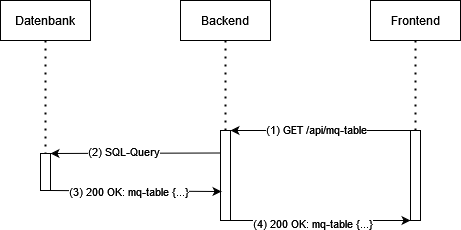
\includegraphics[width=0.8\textwidth]{ressourcen/Ablaufdiagramm}
		\caption[Ablauf eines GET-Requests für das Erstellen der Tabelle]{Ablauf eines GET-Requests für das Erstellen der Tabelle}\label{fig:get-request-for-creation-of-table}
	\end{center}
\end{figure}

Folgende Schritte werden im Ablaufdiagramm durchgeführt.
\begin{enumerate}
	\item Das Frontend sendet einen GET-Request für alle Message-Queues um sie anschliessend in der Tabelle darzustellen.
	\item Das Backend empfängt diesen Request und führt eine SQL-Query aus um die entsprechenden Message-Queues zu erhalten. Die SQL-Query filtert bereits alle Spalten heraus die nicht genutzt werden.
	\item Die Datenbank schickt eine gefilterte Liste mit Message-Queues zurück an das Backend.
	\item Das Backend mappt die entsprechenden Daten in Objekte die das Frontend kennt und schickt es an sie.
\end{enumerate}

Danach kann das Frontend die Daten anzeigen.
\newpage
\section{Anforderungen}
Auf Basis der unter  aufgeführten detaillierten Aufgabestellung und den individuellen Beurteilungskriterien wenden die folgenden Anfortderungen definiert. Die Anforderungen sind den folgenden drei Teilbereichen entsprechend gruppiert und bezeichnet.

\paragraph{MA...} Minimalanforderungen
\paragraph{EP...} Erweiterung Pagination
\paragraph{EF...} Erweiterung Filter

\subsection{Minimalanforderungen}
Folgenden funktionale und nicht funktionale Anforderungen sind hier für die Minimalanforderungen aufgelistet.

\textbf{Funktionale Anforderungen}\newline

\noindent \begin{tabular}{|p{3cm}|p{12cm}|}
	\hline
	\textbf{Anforderung}  & \textbf{Beschreibung} \\ \hline
	MA1    & Die neue Seite ist im Web-GUI auffindbar über den Pfad /admin/mq-table-search und übers Menü unter "Business Daten"→"Queue-Messages".     \\ \hline
	MA2    & Die Tabelle beinhaltet maximal 25 Einträge.     \\ \hline
	MA3    & Alle Einträge sind im Fehlerzustand, d.h. MQ\_IN\_STATUS == 3.     \\ \hline
	MA4    & Die tabellarische Darstellung von MQ\_TABLE beinhaltet volgende Spalten: MODIFIED\_AT, MQ\_QUEUE\_ID, JOB\_KEY, MESSAGE\_SHORT / \_LONG, MQ\_IN\_STATUS, MQ\_IN\_STATUS\_STRING und MQ\_IN\_STATUS\_STRING.    \\ \hline
	MA5    & Anhand von MESSAGE\_IS\_SHORT wird entschieden ob MESSAGE\_SHORT oder MESSAGE\_LONG abgefüllt werden soll.     \\ \hline
	MA6    & Im Web-GUI sollen in der tabellarischen Ansicht nur die ersten 50 Zeichen von MESSAGE\_SHORT / \_LONG angezeigt werde.     \\ \hline
	MA7    & Der MQ\_IN\_STATUS wird in textuelle Stati, gemäss ch.ergon.cardx.shared.database.enumeration.MqInStatus, übersetzt.      \\ \hline
	MA8    & Das Kontextmenü beinhaltet eine Aktion für die Anzeige des kompletten Inhalts der Spalte "Nachricht".     \\ \hline
	MA9    & Das Kontextmenü beinhaltet eine Aktion, um einen erneuten Verarbeitungsversuch eines Eintrages anzustossen. D.h. durch das Setzen des MQ\_IN\_STATUS auf 0.     \\ \hline
	MA10    & Die neuen public-Methoden im Admin-Backend sind mit Unit-Tests bzw. SpringBoot-Tests abgedeckt.Eintrag 4     \\ \hline
	MA11    & Es gibt einen Mock-Datensatz für den neuen MqTable-Rest-Service.     \\ \hline
\end{tabular}

\noindent \textbf{Nicht funktionale Anforderungen}\newline

\noindent \begin{tabular}{|p{3cm}|p{12cm}|}
	\hline
	\textbf{Anforderung}  & \textbf{Beschreibung} \\ \hline
	MA12    & Die Seite ist stimmig ins UI eingebaut, bereits exisiterende UI-Komponenten werden wiederverwendet, oder falls nötig erweitert.     \\ \hline
	MA13    & Die Seite wird in kurzer Zeit geladen, notwendiges Filtering wird auf der Datenbank oder dem Server gemacht.     \\ \hline
\end{tabular}

\subsection{Erweiterung: Pagination}
Folgenden funktionale und nicht funktionale Anforderungen sind hier für die Erweiterung Pagination aufgelistet.

\textbf{Funktionale Anforderungen}\newline

\noindent \begin{tabular}{|p{3cm}|p{12cm}|}
	\hline
	\textbf{Anforderung}  & \textbf{Beschreibung} \\ \hline
	EP1    & Es können mittels Pagination auch mehr als 25 Einträge im Web-GUI angeschaut werden.     \\ \hline
	EP2    & Eine Page beinhaltet maximal 25 Einträge.     \\ \hline
	EP3    & Der Pagination-Mechanismus ist durch Unit-Tests bzw. SpringBoot-Tests abgedeckt.     \\ \hline
\end{tabular} \newline

\noindent \textbf{Nicht funktionale Anforderungen}\newline

\noindent \begin{tabular}{|p{3cm}|p{12cm}|}
	\hline
	\textbf{Anforderung}  & \textbf{Beschreibung} \\ \hline
	EP4    & Einzelne Pages werden erst wenn diese gebraucht werden vom Server geladen.     \\ \hline
	EP5    & Die Navigation zwischen den Seiten ist intuitiv und nutzerfreundlich.     \\ \hline
\end{tabular}

\subsection{Erweiterung: Filter}
Folgenden funktionale und nicht funktionale Anforderungen sind hier für die Erweiterung Filter aufgelistet.

\textbf{Funktionale Anforderungen}\newline

\noindent \begin{tabular}{|p{3cm}|p{12cm}|}
	\hline
	\textbf{Anforderung}  & \textbf{Beschreibung} \\ \hline
	EF1    & Es gibt folgende Filter-Kriterien: Filtern nach MQ\_IN\_STATUS, Filtern mittels Begriffen im Nachrichteninhalt und Filtern nach «Datum von» und «Datum bis»     \\ \hline
	EF2    & Bei Verwendung mehrerer Filter werden diese mittels logischem UND verknüpft.     \\ \hline
	EF3    & Die Filter-Werte können einfach aus dem Web-UI gesetzt werden.     \\ \hline
	EF4    & Die Filterung passiert im Hintergrund, d.h. auf der Datenbank und/oder dem Server.     \\ \hline
	EF5    & Die Einträge sind weiterhin sortiert nach MODIFIED\_DATE.     \\ \hline
	EF6    & Alle Filterkriterien und -werte sind in der URL abgebildet.     \\ \hline
	EF7    & Alle Filter sowie ein Beispiel mit einer Kombination von FIltern sind als Unit-Tests bzw. SpringBoot-Tests abgedeckt.     \\ \hline
\end{tabular}\newline

\newpage
\noindent \textbf{Nicht funktionale Anforderungen}\newline

\noindent \begin{tabular}{|p{3cm}|p{12cm}|}
	\hline
	\textbf{Anforderung}  & \textbf{Beschreibung} \\ \hline
	EF8    & Alle Filterkriterien und -werte sind in der URL abgebildet, um das Speichern und Teilen der Filter zu vereinfachen.     \\ \hline
\end{tabular}

\newpage
    \chapter{Planen}\label{ch:planen}
Dieses Kapitel zeigt die in der IPERKA-Phase «Planen» durchgeführten Arbeiten auf. In dieser Phase werden basierend auf den Anforderungen Arbeitspakete definiert und in einem Zeitplan auf die zehn Probe-IPA Tage aufgeteilt. Zudem werden Lösungskonzepte für die Umsetzung der Seite Business Daten erarbeitet und ein Testkonzept erstellt.

\section{Arbeitspakete}
Die gesamte Arbeit der Probe-IPA wird in Arbeitspakete aufgeteilt. Die Arbeitspakete bestehen aus einer zugehörigen Nummer, einem Namen, dem geschätzten Aufwand und ein erwartetes Ergebnis. In den geschätzten Aufwand sind Zeitreservern mit einberechnet, sodass unvorhergesehenes kompensiert werden kann. Da der Zeitplan in 2-Stunden-Blöcke aufgeteilt ist, wird der geringste Aufwand 2 Stunden sein und im zweier Takt nach oben gehen.

Die Arbeitspakete sind nach der Projektmanagementmethode IPERKA gegliedert. Probe-IPA-spezifische Arbeiten, wie die Expertenbesuche oder das Erstellen des Anhangs, die ausserhalb der eigentlichen Projekts stehen, werden unter «Rahmenaufgaben» aufgeführt.
\subsection{Informieren}
Folgende Arbeitspakete gehören zu der IPERKA-Phase «Informieren».

\begin{longtable}{p{.3\textwidth}|p{.65\textwidth}}
	\hline
	\textbf{Nummer}                 & \textbf{1.1}            \\
	\hline
	\textbf{Name}   				& Projektumfeld analysieren und beschreiben                  \\
	\hline
	\textbf{Geschätzter Aufwand}    & 2h                                    \\
	\hline
	\textbf{Erwartetes Ergebnis}    & Die Aufgabestellung ist beschrieben und für den Lernenden ist der Auftrag klar. Der Lernende kennt das Projektumfeld und hat es dokumentiert.                                    \\
	\hline
\end{longtable}\label{tab:informieren-1.1}

\begin{longtable}{p{.3\textwidth}|p{.65\textwidth}}
	\hline
	\textbf{Nummer}                 & \textbf{1.2}            \\
	\hline
	\textbf{Name}   				& Anforderungen definieren                  \\
	\hline
	\textbf{Geschätzter Aufwand}    & 2h                                    \\
	\hline
	\textbf{Erwartetes Ergebnis}    & Die Anforderungen werden klar definiert und unterteilt in funktionale und nicht funktionale Anforderungen.                                    \\
	\hline
\end{longtable}\label{tab:informieren-1.2}

\subsection{Planen}
Folgende Arbeitspakete gehören zu der IPERKA-Phase «Planen».

\begin{longtable}{p{.3\textwidth}|p{.65\textwidth}}
	\hline
	\textbf{Nummer}                 & \textbf{2.1}            \\
	\hline
	\textbf{Name}   				& Arbeitspakete definieren                  \\
	\hline
	\textbf{Geschätzter Aufwand}    & 4h                                    \\
	\hline
	\textbf{Erwartetes Ergebnis}    & Die gesamten Arbeitspakete sind definiert und nummeriert nach den Phasen von IPERKA.                                    \\
	\hline
\end{longtable}\label{tab:planen-2.1}

\begin{longtable}{p{.3\textwidth}|p{.65\textwidth}}
	\hline
	\textbf{Nummer}                 & \textbf{2.2}            \\
	\hline
	\textbf{Name}   				& Zeitplan erstellen                  \\
	\hline
	\textbf{Geschätzter Aufwand}    & 2h                                    \\
	\hline
	\textbf{Erwartetes Ergebnis}    & Der Zeitplan wird mithilfe der Arbeitspakete erstellt und die bereits erfüllten Aufgaben werden entsprechend markiert.                                    \\
	\hline
\end{longtable}\label{tab:planen-2.2}

\begin{longtable}{p{.3\textwidth}|p{.65\textwidth}}
	\hline
	\textbf{Nummer}                 & \textbf{2.3}            \\
	\hline
	\textbf{Name}   				& Lösungskonzept für die Struktur des Backends                  \\
	\hline
	\textbf{Geschätzter Aufwand}    & 2h                                    \\
	\hline
	\textbf{Erwartetes Ergebnis}    & Ein Lösungskonzept für die Struktur im Backend wird erarbeitet und dokumentiert.                                    \\
	\hline
\end{longtable}\label{tab:planen-2.3}

\begin{longtable}{p{.3\textwidth}|p{.65\textwidth}}
	\hline
	\textbf{Nummer}                 & \textbf{2.4}            \\
	\hline
	\textbf{Name}   				& Lösungskonzept für die Struktur vom Frontend                  \\
	\hline
	\textbf{Geschätzter Aufwand}    & 2h                                    \\
	\hline
	\textbf{Erwartetes Ergebnis}    & Ein Lösungskonzept für die Struktur im Frontend wird erarbeitet und dokumentiert.                                    \\
	\hline
\end{longtable}\label{tab:planen-2.4}

\begin{longtable}{p{.3\textwidth}|p{.65\textwidth}}
	\hline
	\textbf{Nummer}                 & \textbf{2.5}            \\
	\hline
	\textbf{Name}   				& Lösungskonzept für die Struktur von einer Erweiterung                  \\
	\hline
	\textbf{Geschätzter Aufwand}    & 4h                                    \\
	\hline
	\textbf{Erwartetes Ergebnis}    & Der Lernende entscheidet sich zwischen einer der beiden Erweiterungen und erarbeitet für dieses ein Lösungskonzept und dokumentiert diese anschliessend.                                    \\
	\hline
\end{longtable}\label{tab:planen-2.5}

\begin{longtable}{p{.3\textwidth}|p{.65\textwidth}}
	\hline
	\textbf{Nummer}                 & \textbf{2.6}            \\
	\hline
	\textbf{Name}   				& Testkonzept erstellen                  \\
	\hline
	\textbf{Geschätzter Aufwand}    & 4h                                    \\
	\hline
	\textbf{Erwartetes Ergebnis}    & Ein Testkonzept wird erarbeitet. Die zu schreibenden Tests und Testergebnisse sind definiert.                                    \\
	\hline
\end{longtable}\label{tab:planen-2.6}

\subsection{Entscheiden}
Folgende Arbeitspakete gehören zu der IPERKA-Phase «Entscheiden».

\begin{longtable}{p{.3\textwidth}|p{.65\textwidth}}
	\hline
	\textbf{Nummer}                 & \textbf{3.1}            \\
	\hline
	\textbf{Name}   				& Lösungsvarianten evaluieren                  \\
	\hline
	\textbf{Geschätzter Aufwand}    & 4h                                    \\
	\hline
	\textbf{Erwartetes Ergebnis}    & Mögliche Lösungsvarianten wurden evaluiert und die umzusetzende Lösungsvariante ist definiert.                                    \\
	\hline
\end{longtable}\label{tab:entscheiden-3.1}

\subsection{Realisieren}
Folgende Arbeitspakete gehören zu der IPERKA-Phase «Realisieren».

\begin{longtable}{p{.3\textwidth}|p{.65\textwidth}}
	\hline
	\textbf{Nummer}                 & \textbf{4.1}            \\
	\hline
	\textbf{Name}   				& Endpoints für Mindestanforderungen erstellen                  \\
	\hline
	\textbf{Geschätzter Aufwand}    & 4h                                    \\
	\hline
	\textbf{Erwartetes Ergebnis}    & Die Endpoints für die Mindestanforderungen werden erstellt, sodass das Frontend alle Daten, die es braucht, und nur die, die es braucht, bekommt.                                    \\
	\hline
\end{longtable}\label{tab:realisieren-4.1}

\begin{longtable}{p{.3\textwidth}|p{.65\textwidth}}
	\hline
	\textbf{Nummer}                 & \textbf{4.2}            \\
	\hline
	\textbf{Name}   				& Seite und Tabelle im Frontend erstellen                  \\
	\hline
	\textbf{Geschätzter Aufwand}    & 4h                                    \\
	\hline
	\textbf{Erwartetes Ergebnis}    & Die Seite ist mit der entsprechenden URL und im Menü unter Business Daten → Queue-Messages (eingehend) erreichbar. Die Tabelle ist stimmig ins UI eingebaut und entspricht der tabellarischen Darstellung.                                    \\
	\hline
\end{longtable}\label{tab:realisieren-4.2}

\begin{longtable}{p{.3\textwidth}|p{.65\textwidth}}
	\hline
	\textbf{Nummer}                 & \textbf{4.3}            \\
	\hline
	\textbf{Name}   				& Endpoints für Erweiterung erstellen                  \\
	\hline
	\textbf{Geschätzter Aufwand}    & 4h                                    \\
	\hline
	\textbf{Erwartetes Ergebnis}    & Die Endpoints für die Erweiterung werden erstellt, sodass das Frontend alle Daten, die es braucht, und nur die, die es braucht, bekommt.                                    \\
	\hline
\end{longtable}\label{tab:realisieren-4.3}

\begin{longtable}{p{.3\textwidth}|p{.65\textwidth}}
	\hline
	\textbf{Nummer}                 & \textbf{4.4}            \\
	\hline
	\textbf{Name}   				& Erweiterung in die Tabelle integrieren                  \\
	\hline
	\textbf{Geschätzter Aufwand}    & 4h                                    \\
	\hline
	\textbf{Erwartetes Ergebnis}    & Die Erweiterung wird im Frontend in die Tabelle integriert. Das Design der Erweiterung muss stimmig zu der Tabelle und der Seite eingebaut werden.                                    \\
	\hline
\end{longtable}\label{tab:realisieren-4.4}

\begin{longtable}{p{.3\textwidth}|p{.65\textwidth}}
	\hline
	\textbf{Nummer}                 & \textbf{4.5}            \\
	\hline
	\textbf{Name}   				& Release Notes schreiben                  \\
	\hline
	\textbf{Geschätzter Aufwand}    & 1h                                    \\
	\hline
	\textbf{Erwartetes Ergebnis}    & Für die neue Tabelle werden Release Notes geschrieben, um die Tabelle und die Erweiterung zu beschreiben und zu erklären.                                    \\
	\hline
\end{longtable}\label{tab:realisieren-4.5}

\subsection{Kontrollieren}
Folgende Arbeitspakete gehören zu der IPERKA-Phase «Kontrollieren».

\begin{longtable}{p{.3\textwidth}|p{.65\textwidth}}
	\hline
	\textbf{Nummer}                 & \textbf{5.1}            \\
	\hline
	\textbf{Name}   				& Tests                  \\
	\hline
	\textbf{Geschätzter Aufwand}    & 6h                                    \\
	\hline
	\textbf{Erwartetes Ergebnis}    & Das geplante Testkonzept wird umgesetzt und bei Bedarf ergänzt.                                    \\
	\hline
\end{longtable}\label{tab:kontrollieren-5.1}

\begin{longtable}{p{.3\textwidth}|p{.65\textwidth}}
	\hline
	\textbf{Nummer}                 & \textbf{5.2}            \\
	\hline
	\textbf{Name}   				& Codequalität prüfen                  \\
	\hline
	\textbf{Geschätzter Aufwand}    & 2h                                    \\
	\hline
	\textbf{Erwartetes Ergebnis}    & Die Codequalität wird mithilfe der Jenkins-Pipeline überprüft und bei Bedarf überarbeitet.                                    \\
	\hline
\end{longtable}\label{tab:kontrollieren-5.2}

\begin{longtable}{p{.3\textwidth}|p{.65\textwidth}}
	\hline
	\textbf{Nummer}                 & \textbf{5.3}            \\
	\hline
	\textbf{Name}   				& Dokumentation finalisieren                  \\
	\hline
	\textbf{Geschätzter Aufwand}    & 12h                                    \\
	\hline
	\textbf{Erwartetes Ergebnis}    & Die Dokumentation ist nachvollziehbar und verständlich. Das Dokument wird nach Schreibfehlern durchsucht und verbessert, sodass zu diesem Zeitpunkt fast bis gar keine mehr übrig sind. Die Struktur ist einheitlich und Unschönheiten wurden behoben.                                    \\
	\hline
\end{longtable}\label{tab:kontrollieren-5.3}

\subsection{Auswerten}
Folgende Arbeitspakete gehören zu der IPERKA-Phase «Auswerten».

\begin{longtable}{p{.3\textwidth}|p{.65\textwidth}}
	\hline
	\textbf{Nummer}                 & \textbf{6.1}            \\
	\hline
	\textbf{Name}   				& Kurzfassung schreiben                  \\
	\hline
	\textbf{Geschätzter Aufwand}    & 2h                                    \\
	\hline
	\textbf{Erwartetes Ergebnis}    & Das Projekt wird in einer Kurzfassung zusammengefasst.                                    \\
	\hline
\end{longtable}\label{tab:auswerten-6.1}

\begin{longtable}{p{.3\textwidth}|p{.65\textwidth}}
	\hline
	\textbf{Nummer}                 & \textbf{6.2}            \\
	\hline
	\textbf{Name}   				& Reflexion schreiben                  \\
	\hline
	\textbf{Geschätzter Aufwand}    & 2h                                    \\
	\hline
	\textbf{Erwartetes Ergebnis}    & Das Projekt wird vom Lernenden reflektiert und dokumentiert.                                    \\
	\hline
\end{longtable}\label{tab:auswerten-6.2}

\subsection{Rahmenaufgaben}
Folgende Arbeitspakete gehören zu den Rahmenaufgaben.

\begin{longtable}{p{.3\textwidth}|p{.65\textwidth}}
	\hline
	\textbf{Nummer}                 & \textbf{7.1}            \\
	\hline
	\textbf{Name}   				& Projektstruktur aufsetzen                  \\
	\hline
	\textbf{Geschätzter Aufwand}    & 2h                                    \\
	\hline
	\textbf{Erwartetes Ergebnis}    & Aufbau des Gerüstes des \LaTeX Berichtes, welches die Titelseite, ein Glossar, das Quellenverzeichnis und ein Abbildungsverzeichnis beinhaltet. Ein Git-Repository wird für die Dokumentation aufgesetzt.                                    \\
	\hline
\end{longtable}\label{tab:auswerten-7.1}

\begin{longtable}{p{.3\textwidth}|p{.65\textwidth}}
	\hline
	\textbf{Nummer}                 & \textbf{7.2}            \\
	\hline
	\textbf{Name}   				& Aufgabenstellung und Rahmenbedingungen beschreiben                  \\
	\hline
	\textbf{Geschätzter Aufwand}    & 2h                                    \\
	\hline
	\textbf{Erwartetes Ergebnis}    & Die Aufgabenstellung und Rahmenbedingungen hat der Lernende verstanden und beschreibt sie nochmals um dies zu bestätigen.                                    \\
	\hline
\end{longtable}\label{tab:rahmenaufgaben-7.2}

\begin{longtable}{p{.3\textwidth}|p{.65\textwidth}}
	\hline
	\textbf{Nummer}                 & \textbf{7.3}            \\
	\hline
	\textbf{Name}   				& Projektmanagementmethoden definieren                  \\
	\hline
	\textbf{Geschätzter Aufwand}    & 2h                                    \\
	\hline
	\textbf{Erwartetes Ergebnis}    & Eine Projektmanagementmethode wird definiert und durch eine andere wird erläutert, warum sie gewählt wird.                                    \\
	\hline
\end{longtable}\label{tab:rahmenaufgaben-7.3}

\begin{longtable}{p{.3\textwidth}|p{.65\textwidth}}
	\hline
	\textbf{Nummer}                 & \textbf{7.4}            \\
	\hline
	\textbf{Name}   				& Expertenbesuche                  \\
	\hline
	\textbf{Geschätzter Aufwand}    & 2h                                    \\
	\hline
	\textbf{Erwartetes Ergebnis}    & Die Expertenbesuche werden erfolgreich geplant und durchgeführt. Wichtige Informationen bezüglich der Besuche werden an passenden Plätzen erwähnt und dokumentiert.                                    \\
	\hline
\end{longtable}\label{tab:rahmenaufgaben-7.4}

\begin{longtable}{p{.3\textwidth}|p{.65\textwidth}}
	\hline
	\textbf{Nummer}                 & \textbf{7.5}            \\
	\hline
	\textbf{Name}   				& Anhang erstellen                  \\
	\hline
	\textbf{Geschätzter Aufwand}    & 4h                                    \\
	\hline
	\textbf{Erwartetes Ergebnis}    & Ein Anhang mit allen gemachten Änderungen am Quellcode ist dokumentiert und klar von dem unveränderten Code unterscheidbar.                                    \\
	\hline
\end{longtable}\label{tab:rahmenaufgaben-7.5}

\newpage

\section{Lösungskonzept für die Struktur vom Backend}
In diesem Abschnitt wir das Lösungskonzept für einen Teil der unter \ref{ch:minimalanforderungen} definierten Anforderungen beschrieben.

\subsection{Erstellung der Endpunkte}
Im Backend existieren noch keine Endpunkte für die Message-Queues, um sie im Frontend darzustellen. Deshalb müssen diese neu implementiert werden. Die Endpoints werden in einer Service-Klasse erstellt, welche von einem Interface implementiert wird. Die Standardfunktionen, wie GET oder UPDATE, sind bereits im Interface definiert und müssen so nur noch in der Service-Klasse implementiert werden. Der Grund für das Interface ist, dass das Interface für die Service-Klasse und die Mock-Service-Klasse genutzte werden kann und beide Klassen die gleichen Funktionen haben aber mit einer unterschiedlichen Implementierung.
Der Zugriff auf die Datenbank erfolgt in der Klasse ...

\newpage
    \chapter{Entscheiden}\label{ch:entscheiden}
\newpage
    \chapter{Realisieren}\label{ch:realisieren}
Dieses Kapitel zeigt die in der IPERKA-Phase «Realisieren» durchgeführten Arbeiten auf. In dieser Phase wird beschrieben wie der Lernende die Aufgabe umgesetzt hat und spricht Probleme bei der Umsetzung an.

\section{Endpoints für die Mindestanforderungen erstellen}
Die Reihenfolge, welche für diesen Abschnitt folgt, ist die Reihenfolge in der Implementiert wurde.

\subsection{MqInDTO}
Die Implementierung wurde mit der Erstellung von der MqInDto.java Klasse gestartet. Diese Klasse wird öfter in anderen Klassen verwendet und ist aus diesem Grund ein guter Startpunkt. Sie wurde mithilfe der MqOutDto.java Klasse als Beispiel erstellt, um die Konsistenz zwischen den verschiedenen DTO-Klassen beizubehalten. Sie beinhaltet mehrere Annotationen, um den Code kurz zu halten und Zeit bei der Implementation zu sparen:
\paragraph{@Data} \footnote{\url{https://projectlombok.org/features/Data}} generiert Getter, Setter und mehr .
\paragraph{@SuperBuilder} \footnote{\url{https://projectlombok.org/features/experimental/SuperBuilder}} erstellt ein Builder, welcher auch Felder von einer Superklasse verwenden kann.
\paragraph{@NoArgsConstructor} \footnote{\url{https://projectlombok.org/features/constructor}} generiert einen Konstruktor ohne Parameter.
\paragraph{@Schema} \footnote{\url{https://www.baeldung.com/swagger-parameter-vs-schema}} für die Kontrolle von spezifischen Definitionen wie Beschreibung oder Beispiele.
\paragraph{@NotNull} \footnote{\url{https://www.baeldung.com/java-notnull-method-parameter}} stellt sich, dass das Feld nicht «null» ist.\newline

\noindent Anschliessend wurden die Felder erstellt, mit den oben entsprechenden genannten Annotationen, die für die Tabelle im Frontend genutzt werden.

\subsection{MqInMapper}
Die Klasse MqInMapper.java hat die Annotation @Component, sodass Springboot diese Klasse instanziieren und sie mit allen angegebenen Abhängigkeiten injizieren kann.

Zwei Funktionen namens toMqInDto() und listToMqInDto() wurden in dieser Klasse erstellt. Die erste Funktion macht ein Mapping von MqTablePC (die ursprüngliche MqInPC-Klasse) zu MqInDto. Sie verwendet den Builder von der zuvor genutzten Annotation @SuperBuilder. Die zweite Funktion ruft die erste mithilfe von einem Stream auf. Der Stream wird verwendet, um jedes Element der Liste mit der Funktion toMqInDto aufzurufen. Dies wird mit .map() gemacht. Der Stream ermöglicht es, diese Aufgabe in einer kurzen Zeile zu schreiben, anstatt mit einem Loop jedes einzele Element der Liste hervorzuholen, zu mappen und anschliessend in einer zweiten Liste zu speichen. Die Funktion hat durch das nur insgesammt 3 Zeilen und vereinfacht das lesen.

\begin{verbatim}
	public List<MqInDto> listToMqInDto(List<MqTablePC> listOfMqTablePCs) {
		return listOfMqTablePCs.stream().map(this::toMqInDto).toList();
	}
\end{verbatim}

\subsection{MqInService}
Um die Struktur von eine Service vorzugeben, wurde ein Interface mit dem Namen MqInService erstellt. Dieses Interface wird später für die Klasse MqInServiceImpl.java und MqInServiceMockImpl.java verwendet und beinhaltet im Moment zwei Funktionen für das hervorholen von allen MqTables in der Datenbank und das ausführen von einem neuen Verarbeitungsversuch.

\subsection{MqInServiceImpl}
MqInServiceImpl wird vom Interface MqInService implementiert. Sie wird mit der Annotation @Service für Springboot als Service deklariert. Die Klasse enthält die vom Interface vorgegebene Funktion getMqTables(). Sie ruft eine Funktion von der Klasse MqTableDao (die ursprüngliche MqInDao-Klasse) auf die alle MqTable Einträge mit dem Status «Error» von der Datenbank hervorholt und sie auf 25 Einträge limitiert. Ein ändlicher Vorgehen hat die Funktion executeNewProcessingAttempt() die den Status vom MqIn auf NEW setzt.  

In dieser Klasse wurde auch ein Konstruktor erstellt. Bei dieser Implementierung trat ein Problem auf welches die Applikation nicht starten lies. Bei dem Parameter MqTableDao erschien die Meldung «Could not autowire. No beans of 'MqTableDao' type found.». Das Problem war, dass für die Klasse MqTableDao noch kein Bean erstellt wurde, obwohl die Klasse schon vorher existierte. Das Bean wurde anschliessend in der Klasse WebBackendAdminSpringConfiguration.java erstellt.

\subsection{MqTableDao}
Diese Klasse existierte bereits und war ursprünglich als MqInDao geplant. Durch das mussten nur die Funktionen hinzugefügt werden. Da es ein Interface ist, wurden nur die Namen und die benötigten Parameter hinzugefügt. Es wurden noch keine Bodys implementiert. Ausserdem wurden bei beiden Funktionen ein Kommentar erstellt. Der Kommentar beinhaltet eine kurze Beschreibung der Funktion und was sie zurückgibt. Mithilfe dieses Kommentars kann man jetzt über die Funktion drüberfahren und die Beschreibung wird als kurze Erklärung angezeigt.

\subsection{MqTableHibernateDao}
In der Klasse MqTableHibernateDao wird das Interface MqTableDao implementiert und muss durch das auch die neu erstellte Funktion implementieren.

Die Funktion nutzt einen CriteriaBuilder, um eine SQL-Query zu erstellen. Mit dieser Klasse konnte die Query so generiert werden, dass sie nach Enträgen filtert, die einen MQ\_IN\_STATUS von ERROR, als die Nummer Drei, haben. Die Query wird mithilfe von der Klasse CriteriaQuery bearbeitet und mit der Klasse Root können die einzelnen Spalten hervorgeholt werden, um sie zu vergleichen.

Um die Einträge auf 25 zu limitieren, musste noch die Klasse TypedQuery verwendete werden, welche dies ermöglichte.

\begin{verbatim}
	@Override
	public List<MqTablePC> findAllWithStatusErrorLimitedTo25() {
		CriteriaBuilder cb = getSession().getCriteriaBuilder();
		CriteriaQuery<MqTablePC> query = cb.createQuery(MqTablePC.class);
		Root<MqTablePC> mqTable = query.from(MqTablePC.class);
		
		query.where(
			cb.equal(mqTable.get(FN_MQ_IN_STATUS), ERROR)
		).orderBy(cb.desc(mqTable.get(FN_MODIFIED_AT)));
		
		TypedQuery<MqTablePC> typedQuery = getSession().createQuery(query);
		typedQuery.setMaxResults(25);
		
		return typedQuery.getResultList();
	}
\end{verbatim}

\noindent Für die zweite Funktion wurde ein CriteriaUpdateBuilder verwendet. Die restliche Implementation blieb fast gleich. Die Limitierung wurde entfernt und ein set() hinzugefügt, um den MQ\_IN\_STATUS auf NEW zu setzten.

\subsection{MqInResource}
Die Klasse MqInresource beinhaltet den geplanten Endpoint welcher im Arbeitspaket \ref{tab:realisieren-4.1} beschrieben wurde. Die Klasse wurde mit @RestController annotiert, sodass Spring weiss das diese Klasse Endpoints enthält. Sie hat ausserdem noch @RequestMapping, um den Pfad zu definieren und @RequiredArgsConstructor, welcher en Konstruktor generiert mit allen finalen und nicht-null Feldern.

Der Endpoint selbst hat drei Annotationen:

\paragraph{@GetMapping} \footnote{\url{https://www.geeksforgeeks.org/spring-postmapping-and-getmapping-annotation/}} deklariert diesen Endpoint als ein GET-Request.
\paragraph{@Operation} \footnote{\url{https://www.baeldung.com/swagger-operation-vs-apiresponse}} beschreibt die Funktion von diesem Endpoint.
\paragraph{@RequirePermission} \footnote{Vom Projekt CardX implementiert} stellt die Befugnis von diesem Endpoint ein. \newline

\noindent Der Endpoint selbst greift nur auf die erstellte Funktion in der Klasse MqInService.java zu und Mapped das erhaltene Resultat mithilfe des Mappers bevor er es wieder zurück sendet.

Der zweite Endpoint für das aussführen von einem weiteren Verarbeitungsversuch ist gleich aufgebaut wie der erste mit zwei Unterschieden. Er hat zwei andere Annotationen. Einerseits wurde der @GetMapping mit einem @RequestMapping ersetzt, sodass Spring weiss, dass es die Requests zu den richtigen Endpoints verweisen kann. Ausserdem hat dieser Endpoint ein Parameter namens id. Dieser Parameter wird vom RequestBody befüllt und muss deshalb mit @RequestBody annotiert werden.

\section{Die Seite und Tabelle im Frontend erstellen}

\subsection{Erstellung der Tabelle}\label{ch:creation-of-table}
Für die Erstellung der Tabelle wurde eine mq-in.service.ts-Klasse erstellt. Diese wird für die Requests an das Backend verwendet und beinhaltet die Funktion getAllMqInsLimitedTo25(), um alle MqIns von der Datenbank zu laden, und executeNewProcessingAttempt(id: number), die für die erneute Ausführung von einem Verarbeitungsveruch zuständig ist. Beide Funktionen rufen ihren erstellten Endpoint auf, welcher für das Frontend vom Projekt generiert wurde.

Diese Generierung kann mithilfe der Annotationen bei den entsprechenden Endpoints die HTTP-Requests generieren. Durch die generierte Swagger Datei wird eine zweite JSON-Datei generiert, die alle genötigten Informationen beinhaltet und im Modul Interface als web-backend-admin-api-.json gespeichert wird. Ein Plugin im Frontend nutzt anschliessend diese Datei, um die HTTP-Requests zu generieren.

Die Generierung vereinfachte die Nutzung von HTTP-Requests und hat die entsprechende Implementierung beschleunigt. Die Tabelle für die MqIns wurde durch das schnell erstellt und die ersten Einträge waren sichtbar auf der Seite.

\begin{figure}[H]
	\begin{center}
		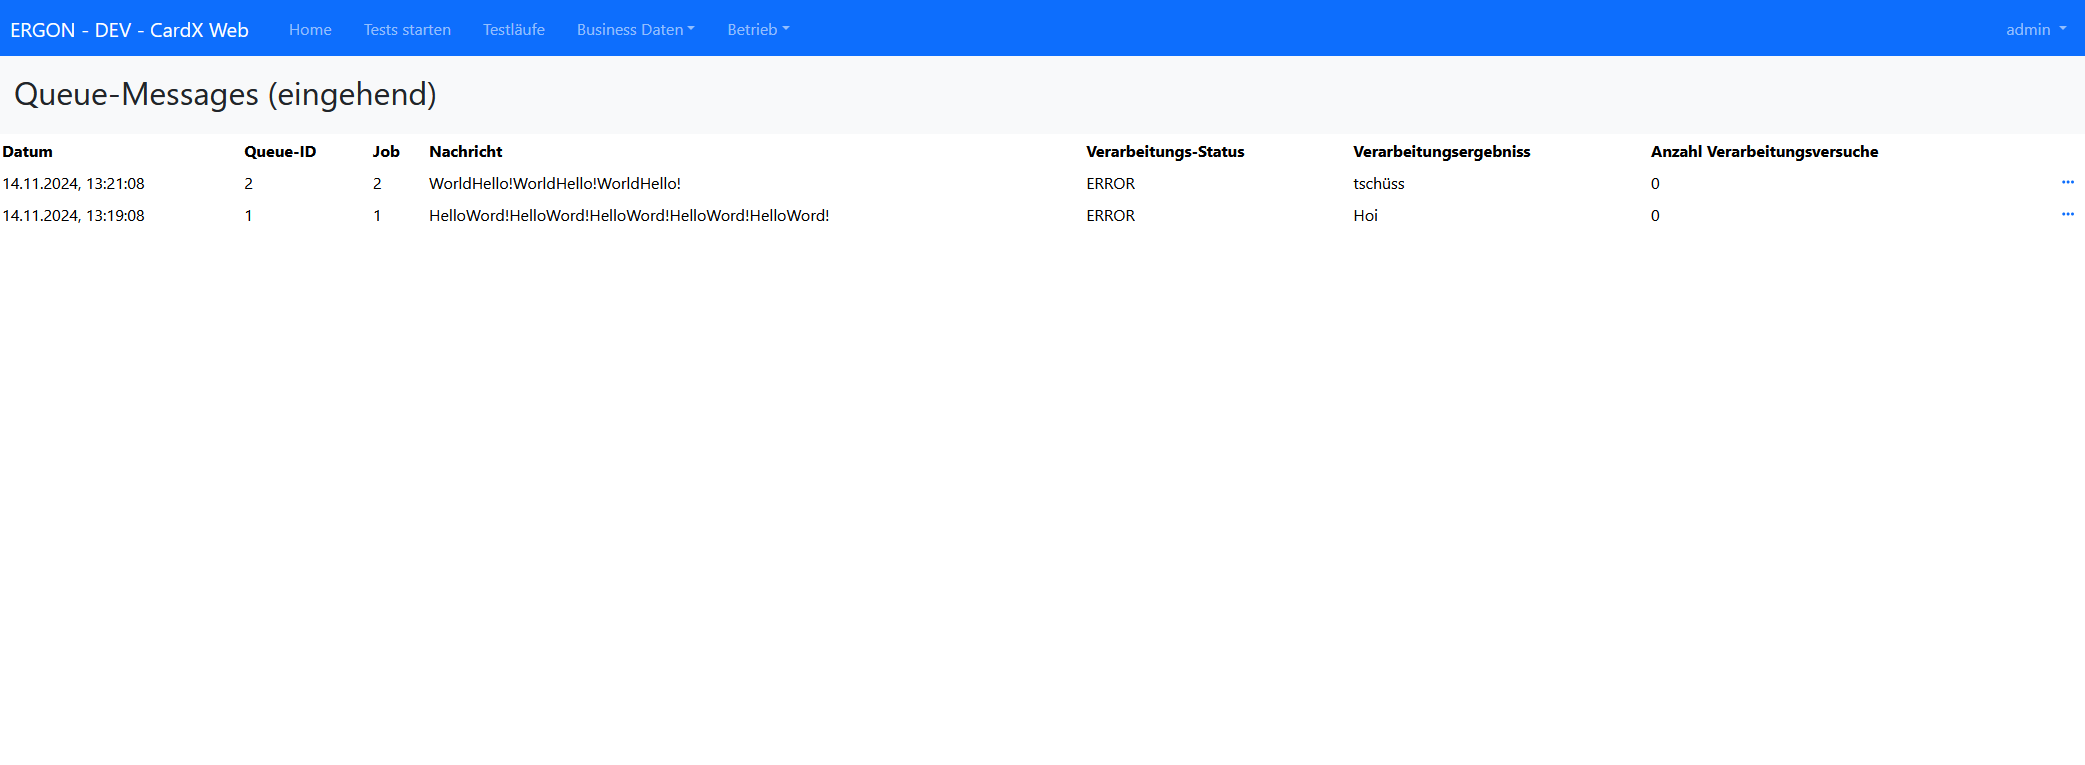
\includegraphics[width=1\textwidth]{ressourcen/4.2_Tabelle}
		\caption[Aktueller Stand der Tabelle]{Aktueller Stand der Tabelle}\label{fig:4.2-tabelle}
	\end{center}
\end{figure}

\subsection{Anzeigen der ganzen Nachricht}
Für das Anzeigen der ganzen Nachricht wurde eine neue Map erstellt, welche als Key die ID des MqIns und als Value einen Boolean enthält. Diese Map wird immer beim Aufruf der Seite gefüllt, nach dem die MqIns geladen wurden. Durch diese Map kann die ganze Nachricht angezeigt und anschliessend wieder verkürzt werden. Die eine Funktion setzt den entsprechenden Wert jedes Mal um, wenn man auf den Knopf «ganze Nachricht anzeigen» oder «Nachricht kürzen» drückt.

\noindent Die kurze Nachricht wird angezeigt:
\begin{figure}[H]
	\begin{center}
		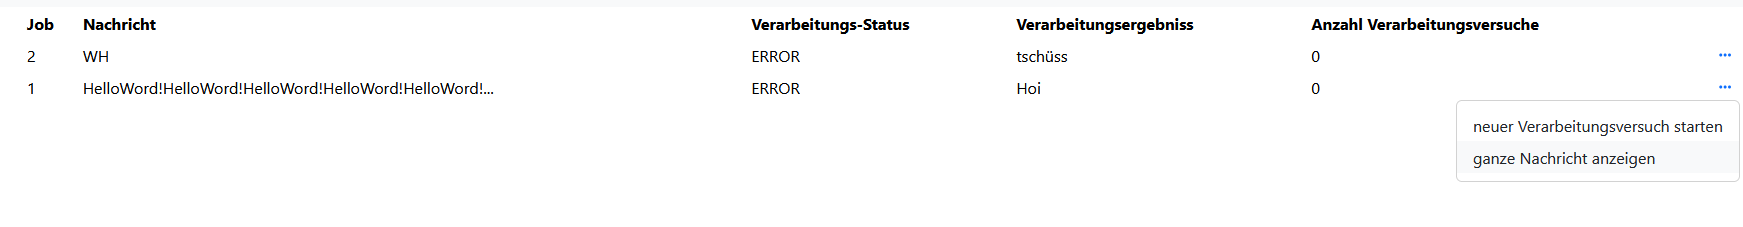
\includegraphics[width=1\textwidth]{ressourcen/Kurze-Nachricht}
		\caption[Gekürzte Nachricht]{Gekürzte Nachricht}\label{fig:show-shortend-version-of-message}
	\end{center}
\end{figure}

\noindent Die ganze Nachricht wird angezeigt:
\begin{figure}[H]
	\begin{center}
		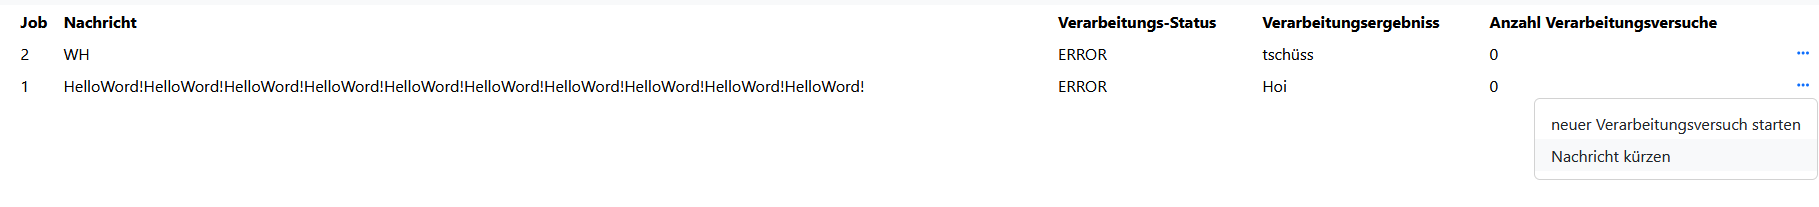
\includegraphics[width=1\textwidth]{ressourcen/Ganze-Nachricht}
		\caption[Ganze Nachricht]{Ganze Nachricht}\label{fig:show-hole-message}
	\end{center}
\end{figure}

\subsection{Erneutes Ausführen vom Verarbeitungsversuch}
Die Implementation für dieses Feature dauerte nicht lange, da, wie oben beschrieben \ref{ch:creation-of-table}, die HTTP-Requests generiert wurden und die Funktion nur noch verknüpft werden musste beim Drücken des Knopfs «neuer Verarbeitungsversuch starten». Dies war schnell gemacht und kostete nur im Backend ein wenig Zeit.

\begin{verbatim}
	private executeNewProcessingAttempt(id: number) {
		this.mqInService.executeNewProcessingAttempt(id)
		.subscribe({
			next: () => {
				this.loadMqIns();
			},
			error: (e: HttpErrorResponse) => {
				throw new ApiHttpErrorResponse('Die Verarbeitung der Queue konnte nicht neu gestartet werden.', e);
			},
		});
	}
\end{verbatim}

\noindent Diese Funktion ruft die Funktion executeNewProcessingAttempt() mit dem Parameter ID auf. Anschliessend führt die Subscribe folgende zwei Aktionen aus:

\paragraph{next:} wird ausgeführt, wenn der HTTP-Request erfolgreich war und die erwarteten Daten bereitgestellt wurden. In diesem Fall wird die Liste neu geladen.
\paragraph{error:} wird ausgeführt, wenn der HTTP-Request nicht erfolgreich war und ein Fehler während der Ausführung auftritt. Hier wird ein Fehler mit einer Nachricht geworfen.\newline

\noindent Danach ist die Backend-Anfrage fertig und war entweder erfolgreich oder nicht.

\section{Endpoints für die Erweiterung Filter erstellen}
Die Reihenfolge, welche für diesen Abschnitt folgt, ist die Reihenfolge in der Implementiert wurde. Die Klassen werden nicht mehr im Detail beschrieben, was oben bereits erklärt wurde.

\subsection{MqInFilterDto}
Um die Datensätze der Datenbank zu filtern, wurde ein weiteres DTO erstellt, um die Filterkriterien vom Frontend zu empfangen. Die Klasse beinhaltet vier Variablen namens status, messageQuery, timestampFrom und timestampTo. Ausserdem sind alle Variablen noch mit der Annotation @Schema beschrieben.

\subsection{MqInService}
Im Interface MqInService wurde wieder eine neue Funktion, getFilteredMqTablePCs(), hinzugefügt. Sie nimmt einen Parameter mit dem Typ MqInFilterQuery, dieser Record wurde in der Klasse MqTableDao hinzugefügt und wird später nochmals genauer erklärt, und gibt eine Liste mit MqTablePCs zurück.

\subsection{MqInServiceImpl}
Die Implementierung der neu erstellten Funktion im Interface MqInService wurde hier implementiert. Die Funktion hat gerade mal eine Zeile Code, die im Interface MqTableDao eine weitere Funktion aufruft.

\subsection{MqTableDao}
Das Interface hat zwei neue Inhalte dazu bekommen.

Einerseits wurde die neue Funktion getFilteredMqTablePCs() deklariert. Sie hat den gleichen Parameter und Rückgabewert wie die Funktion im Interface MqInService.

Und andererseits wurde hier ein neuer Record namens MqTableFilterQuery hinzugefügt. Ein Record ist eine speziele Art von Klasse, die hauptsächlich für datenzentrierte Klassen dient. Die Klasse ist dadurch einfach und prägnant, da sie Funktionen wie Konstruktoren, Getter, toStirng, hashCode oder equals bereits implementiert und sie so nicht erneut geschrieben werden müssen. Die Felder der Klasse werden duch Parameter angegeben. Dieser Record beinhaltet status, messageQuery, timestampFrom und timestampTo als Parameter.

\subsection{MqTableHibernateDao}
Die zuvor deklarierte Funktion getFilteredMqTablePCs() wird hier implementiert. Sie hat ähnliche Variablen wie die anderen Funktionen in dieser Klasse, wie CriteriaBuilder, CriteriaQuery und Root. Was bei dieser Funktion speziel ist, sie hat eine weitere Variable mit dem Typ Predicate. Diese Variable ermöglicht es, eine Liste von Filtern zu erstellen. Da nicht immer alle Filter gesetzt werden, müssten ansonsten mehrere Funktionen erstellt werden. Mit dieser Variable kann man die gesetzten Filter zu der Liste hinzufügen und am Ende die Elemente zu der SQL-Query hinzugefügt werden. Dies hat es also ermöglicht, alle Filter mit einer Funktion zu setzen und so das richtige Resultat zu erhalten.

\begin{verbatim}
	@Override
	public List<MqTablePC> getFilteredMqTablePCs(MqTableFilterQuery filterQuery) {
		CriteriaBuilder cb = getSession().getCriteriaBuilder();
		CriteriaQuery<MqTablePC> query = cb.createQuery(MqTablePC.class);
		Root<MqTablePC> mqTable = query.from(MqTablePC.class);
		List<Predicate> predicates = new ArrayList<>();
		
		Optional.ofNullable(filterQuery.status()) // Einfügen der Filters status
		.ifPresent(status ->
		predicates.add(cb.equal(mqTable.get(FN_MQ_IN_STATUS), status))
		);
		
		Optional.ofNullable(filterQuery.messageQuery()) // Einfügen der Filters messageQuery
		.ifPresent(messageQueue -> {
			String searchTerm = "%" + filterQuery.messageQuery().toLowerCase(Locale.getDefault()) + "%";
			predicates.add(
			cb.or(
			cb.like(cb.lower(mqTable.get(FN_MESSAGE_SHORT).as(String.class)), searchTerm),
			cb.like(cb.lower(mqTable.get(FN_MESSAGE_LONG).as(String.class)), searchTerm)
			)
			);
		});
		
		Optional.ofNullable(filterQuery.timestampFrom()) // Einfügen der Filters timestampFrom
		.ifPresent(timestampFrom ->
		predicates.add(cb.greaterThanOrEqualTo(mqTable.get(FN_MODIFIED_AT), timestampFrom))
		);
		
		Optional.ofNullable(filterQuery.timestampTo()) // Einfügen der Filters timestampTo
		.ifPresent(timestampTo ->
		predicates.add(cb.lessThanOrEqualTo(mqTable.get(FN_MODIFIED_AT), timestampTo))
		);
		
		
		query.select(mqTable)
		.where(cb.and(predicates.toArray(Predicate[]::new)))
		.orderBy(cb.desc(mqTable.get(FN_MODIFIED_AT)));
		
		return getSession().createQuery(query)
		.setMaxResults(25)
		.getResultList();
	}
\end{verbatim}

\section{Die Erweiterung in die Tabelle integrieren}
Durch die grosse Verzögerung während dem implementieren von diesem Teil hat sich der Lernende dazu entschieden die Erweiterung zu pausieren und zuerst mit den restlichen Arbeitspaketen weiter zu mache. Falls am Ende der Probe-IPA noch Zeit übrig ist, wird die Implementierung fortgesetzt. 

Die Reihenfolge, welche für diesen Abschnitt folgt, ist die Reihenfolge in der Implementiert wurde.

\subsection{mq-in-filter-url}
Um die Parameter von der Url für da Filtern zu extrahieren wurde in dieser Klasse eine Funktion getMqInFilterUrlStateFromParams erstellt. Diese Funktion nimmt eine Mapü mit den Parametern. Mit dieser Map wird mithilfe vom Enum MqInFilterUrlKeys alle Werte von der Url hervorgeholt und anschliessend alle Werte, die nichts beinhalten, aus der Liste entfernt. Als Rückgabewert wird MqInFilterUrlState verwendet.

Dieser Typ beinhaltet Keys mit dem Typ MqInFilterUrlKeys und die Werte haben einen Typ String. Dies wird mit einem Record definiert. Durch das hinzufügen des Typs Partial werden die Werte optional und müssen nicht befüllt werden.

\begin{verbatim}
	export enum MqInFilterUrlKeys {
		STATUS = 'status',
		MESSAGE_QUEUE = 'messageQuery',
		TIMESTAMP_FROM = 'timestampFrom',
		TIMESTAMP_TO = 'timestampTo',
	}
	
	export type MqInFilterUrlState = Partial<Record<MqInFilterUrlKeys, string>>;
	
	export function getMqInFilterUrlStateFromParams(params: ParamMap): MqInFilterUrlState {
		const result: MqInFilterUrlState = Object.values(MqInFilterUrlKeys)
		.reduce((state, urlParam) => ({ ...state, [urlParam]: params.get(urlParam) }), {});
		return omitBy(result, isEmpty);
	}
\end{verbatim}

Anschliessend wurde noch ein mapping für den Typ FilterQueryDto erstellt für die Backend-Anfrage.

\subsection{mq-in-filter.component}
Diese Klasse wird für das anzeigen der Filter verwendet. Es wurde ein FormGroup erstellt mit den Filter-Werten, die anfangs einfach Null sind. Der Status jedoch hat den Wert ERROR um den Mindestanforderungen gerecht zu werden, da sie bei der ersten Abfrage nur Elemente mit diesem Wert wollen. Dies wird durch ein ngOnInit() gemacht, da diese Funktion immer als erstes aufgerufen wird, wenn man die Seite aufruft.

Um die Werte von der Url in das Formular einzufügen wurde eine weitere Funktion erstellt, die alle Parameter mit der Hilfe von der zuvor erstellten Funktion getMqInFilterUrlStateFromParams(). Sie speichert die erhaltenen Parameter in einer Variable und setzt anschliessend die FormGroup mit den erhaltenen Werten.

Um eine Filterung durchzuführen werden beim Event submit alle Werte des Filters im Typ MqInFilterUrlState gespeichert und anschliessend für die Elternkomponente bereit gestellt durch ein Event.

Das Endresultat der Implementierten Funktionen und Klassen sieht anschliessend im Web-GUI so aus:

\begin{figure}[H]
	\begin{center}
		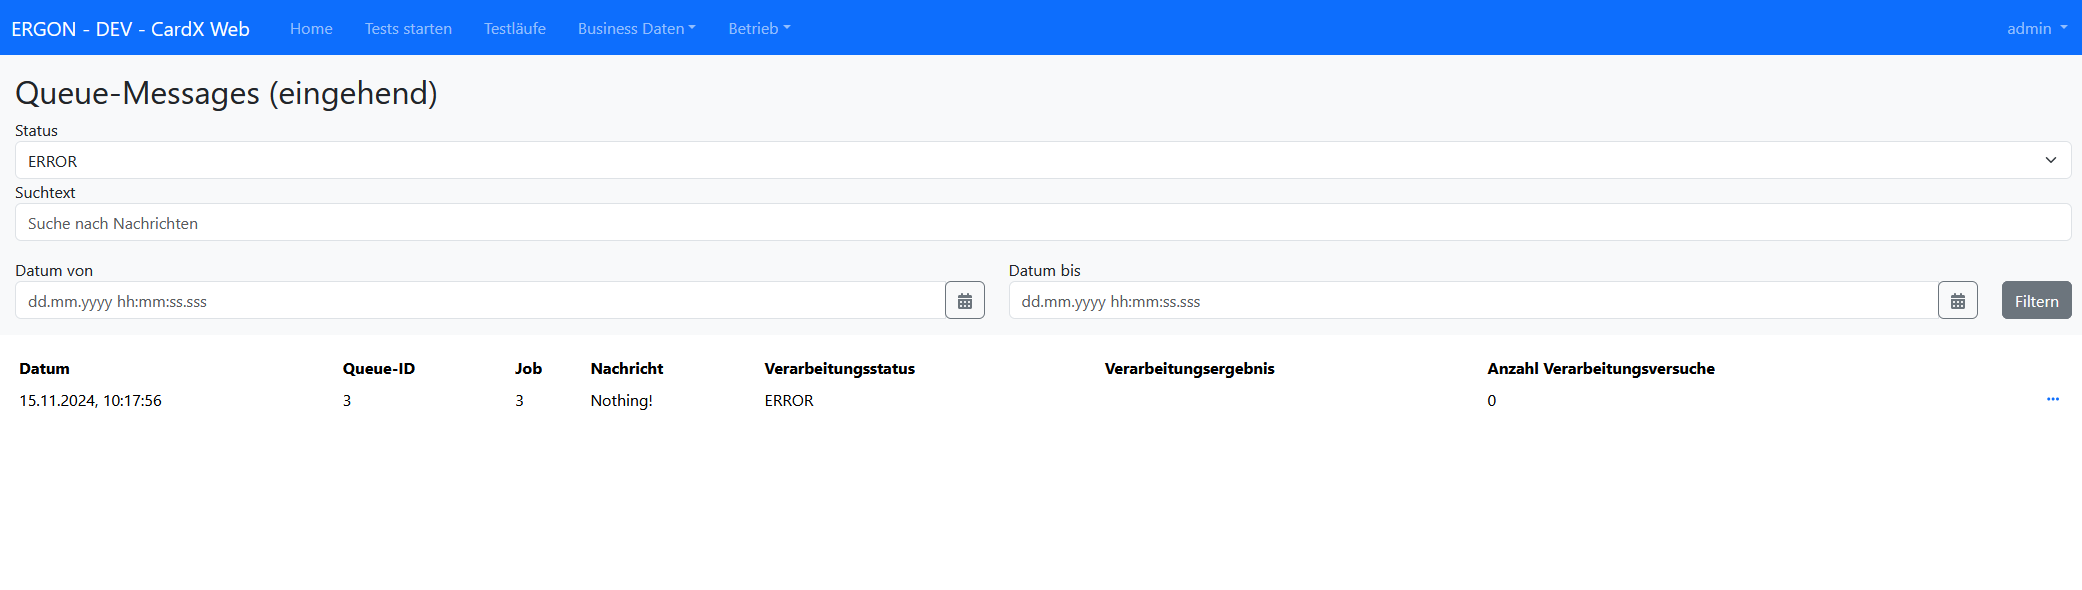
\includegraphics[width=1\textwidth]{ressourcen/Filterung}
		\caption[Der aktuelle Stand des Filters]{Der aktuelle Stand des Filters}\label{fig:filtering-v1}
	\end{center}
\end{figure}

\subsection{Fehlerbeschreibung}
Durch eine Fehler welcher nicht ermittelt werden konnte, wurde die Erweiterung pausiert. Der Fehler erscheint anfangs beim aufrufen der Seite und hat den HTTP-Statuscode 500, was auf einen Server interner Fehler hinweist. Es wurde nicht herrausgefunden was der Fehler war. Mit Debugging wurde versucht den Request im Backend abzufangen und manuell durch die Funktionen zu gehen, aber der Request kam nicht im Backend an. Nach ein paar Stunden Debugging und Fehlersuche wurde entschieden, dass die Implementation der Erweiterung pausiert wird und zu einem späteren Zeitpunkt erneut einen Versucht zu starten mit einem Fachverantwortlichen.

\section{ReleaseNotes schreiben}
Um die Änderungen in den Master mergen zu können muss man ReleaseNotes für das implementierte Jira-Ticket schreiben. Für dieses Ticket wurden folgende ReleaseNotes geschrieben:

\begin{verbatim}
	## Webinterface
	* CARDXDEV-2268 Neue Seite unter Business Daten > Queue Messages (eingehend)
	  hinzugefügt mit einer MqIn-Tabelle.
\end{verbatim}
\newpage
    \chapter{Kontrollieren}\label{ch:kontrollieren}
Dieses Kapitel zeigt die in der IPERKA-Phase «Kontrolieren» durchgeführten Arbeiten auf. In dieser Phase wird beschrieben wie der Lernende die Tests implementiert hat und welche Technologien schlussendlich verwendet wurden.

\section{Allgemein}
Die Tests wurden im entsprechenden Ordner «test» erstellt. In diesem Ordner existieren auch bereits andere Tests und auch Unterkategorien wie configuration, integrationtest, resource, shared und util. Die geplanten Tests wurden in dem Ordner integration und resource erstellt und implementiert. Um die Tests zu schreiben und mit @Test zu deklarieren wurde JUnit \footnote{\url{https://junit.org/junit5/}} verwendet.

\section{Integration-Tests}
Für die Erstellung der Daten wurde ein interne Klasse von dem CardX-Projekt verwendet. Die Klasse trägt den Namen «A» und ermöglicht es von vielen PCs im Projekt ein Objekt zu erstellen, welches anschliessend in einer Datenbank gespeichert wird und das erstellte Objekt zurückgegeben wird. Diese Klasse wurde verwendet um verschiedene MqTablePC-Objekte zu erstellen und sie daraufhin zu für die Endpoints zu nutzen.

\subsection{testGetAllMqIns}
Dieser Test überprüft die Funktionalität vom GET-Request um alle MqIns mit dem Status ERROR hervorzuholen. Die Objekte werden mithilfe von einer erstellten Funktion erstellt und anschliessend ein GET-Request auf den zu testenden Endoint gemacht. Dieser Request wird mit WebCliend gemacht der von dem Springframework zur verfügung gestellt wird.

\begin{verbatim}
	MqInDto[] mqInDtos = WebClient.create("http://localhost:" + getPort())
	.get()
	.uri(PATH)
	.retrieve()
	.bodyToMono(MqInDto[].class)
	.block();
\end{verbatim}

\paragraph{.get()} deklariert den Request als GET-Request.
\paragraph{.uri(PATH)} wird verwendet um den Pfad des Endpoints anzugeben.
\paragraph{.retrieve()} wird im zusammenhang mit bodyToMono() verwendet.
\paragraph{.bodyToMono(MqInDto[].class)} stellt sich, dass der Rückgabewert eine Liste von MqInDtos ist.
\paragraph{.block()} blockiert alle synchonen Requests bis dieser Request abgeschlossen ist.

Das Resultat des Requests wurde anschliessend mit «assertNotNull» und «asserThat» überprüft auf Richtigkeit. Zuerst wurde geschaut ob die erhaltenen Liste null ist und anschliessend die Länge und den Inhalt auf Korrektheit geprüft.

\subsection{testExecuteNewProcessingAttempt}
Das Verfahren der Implementierung dieses Tests sind fast gleich. Der Unterschied ist, dass zweimal ein Get-Request ausgeführt wird. Das erste Mal, um den ursprünglichen Stand der Datenbank hervorzuholen und ein zweites Mal nach dem der PUT-Request getätigt wurde, um zu überprüfen ob das Objekt überschrieben wurde.

Der PUT-Request ist gleich aufgebaut wie die GET-Requests mit zwei kleinen unterschieden. Es wurde ein Body hinzugefügt mit der id des zu überschreibenden Objekts und das .get() wurde mit .put() ersetzt.

\begin{verbatim}
	Long idOfMqIn = Arrays.stream(mqInsBevorUpdate).findFirst().get().getId();
	Integer response = WebClient.create("http://localhost:" + getPort())
	.put()
	.uri(PATH + "/")
	.body(Mono.just(idOfMqIn), Long.class)
	.retrieve()
	.bodyToMono(Integer.class)
	.block();
\end{verbatim}

\subsection{testGetFilteredMqInEntries}
Für das Testen der Filter-Requests wurde ein MqInFilterDto Objekt erstellt und mit den folgenden Filtern befüllt:

\begin{itemize}
	\item Nachricht: mqTable3
	\item Status: NEW
	\item Datum bis: 202.11.20TT23:00:00
\end{itemize}

Das Filterergebnis sollte alles heraus filtern bis auf ein Element. Dieses wurde anschliessend auf die Richtigkeit des Status, der Nachricht und dem Datum bis.

\begin{verbatim}
	@Test
	void testGetFilteredMqInEntries() {
		setupDB();
		
		MqInFilterDto filter = new MqInFilterDto();
		filter.setMessageQuery("mqTable3");
		filter.setStatus("NEW");
		filter.setTimestampTo(LocalDateTime.of(2024, 11, 20, 23, 0, 0).toString());
		
		MqInDto[] mqIns = WebClient.create("http://localhost:" + getPort())
		.put()
		.uri(PATH + "/filtered")
		.body(Mono.just(filter), MqInFilterDto.class)
		.retrieve()
		.bodyToMono(MqInDto[].class)
		.block();
		
		assertNotNull(mqIns);
		assertThat(mqIns.length).isEqualTo(1);
		assertThat(mqIns[0].getMqInStatus()).isEqualTo(MqInStatus.NEW);
		assertThat(mqIns[0].getMessage()).isEqualTo("mqTable3");
	}
\end{verbatim}

\section{Unit-Tests}
Um die Daten für das Testing bereitzustellen, wurde ein Klasse MqInMock erstellt. Diese Klasse beinhaltet ein paar Funktionen welche ein, mehrere oder verschiedene MqTablePCs zurück gibt.

\subsection{testMappingWithSinglePC}
Dieser Test überprüft die Funktion toMqInDto(MqTablePC mqTablePC) welche aus einem MqTablePC-Objekt ein MqInDto-Objekt mapped. Der Test selbst ist einfach aufgebaut. Er erstellt zuerst das zu mappende Objekt und gibt es anschliessend als Parameter beim Aufruf der Funktion mit. Danach wird mithilfe von assertNotNull() und assertThat() auf überprüft ob es existiert und ob alle Werte richtig gesetzt worden sind.

\subsection{testMappingWithMultiplePCs}
Hier wird ein ähnlicher Aublauf verwendet wie beim Test zuvor. Der Unterschied liegt aber dabei, dass die Funktion listToMqInDto(List<MqTablePc> listOfMqTablePCs) aufgerufen wird und eine Liste mitgegeben wird. Bei der Überprüfung wird ausserdem durch die erhaltene Liste iteriert und bei jedem einzelnem Element die erwarteten Werte überprüft.

\begin{verbatim}
	@Test
	void testMappingWithMultiplePCs() {
		// given
		List<MqTablePC> mqTablePCs = MqInMocks.createEveryStatusTypeOfMqTablePC();
		
		// when
		List<MqInDto> mqInDtos = mapper.listToMqInDto(mqTablePCs);
		
		// then
		assertNotNull(mqInDtos);
		for (MqTablePC mqTablePC : mqTablePCs) {
			MqInDto mqInDto = mqInDtos.stream().filter(mqIn -> mqIn.getId() == mqTablePC.getId()).findFirst().get();
			assertNotNull(mqInDto);
			assertThat(mqInDto.getId()).isEqualTo(mqTablePC.getId());
			assertThat(mqInDto.getMessage()).isEqualTo(mqTablePC.getMessage());
			assertThat(mqInDto.getJobKey()).isEqualTo(mqTablePC.getJobKey());
			assertThat(mqInDto.getModifiedAt()).isEqualTo(mqTablePC.getModifiedAt());
			assertThat(mqInDto.getMqQueueId()).isEqualTo(mqTablePC.getMqQueueId());
			assertThat(mqInDto.getProcessedCnt()).isEqualTo(mqTablePC.getProcessedCnt());
			assertThat(mqInDto.getMqInStatusString()).isEqualTo(mqTablePC.getMqInStatusString());
			assertThat(mqInDto.getMqInStatus()).isEqualTo(mqTablePC.getMqInStatus());
		}
	}
\end{verbatim}

\subsection{testMappingOfMqInFilterDto}
Dieser Teste ist gleich aufgebaut wie der erste Test. Die verwendeten Klassen sind andere. Vom gröberen Aufbau ist es aber der gleiche Test einfach für eine andere Funktion. Er überprüft die funktionalität der toMqTableFilterQuery Funktion für das Filter der Elemente.

\begin{verbatim}
	@Test
	void testMappingOfMqInFilterDto() {
		// given
		MqInFilterDto filterDto = MqInMocks.createMqInFilterDto();
		
		// when
		MqTableDao.MqTableFilterQuery result = mapper.toMqTableFilterQuery(filterDto);
		
		// then
		assertNotNull(result);
		assertThat(result.status()).isEqualTo(MqInStatus.ERROR);
		assertThat(result.messageQuery()).isEqualTo("mqTable1");
		assertThat(result.timestampFrom()).isEqualTo(OffsetDateTime.of(2024, 11, 20, 10, 0, 0, 0, ZoneOffset.ofHours(1)));
		assertThat(result.timestampTo()).isEqualTo(OffsetDateTime.of(2024, 11, 20, 20, 0, 0, 0, ZoneOffset.ofHours(1)));
	}
\end{verbatim}

\section{Codequalität prüfen}
Für die Überprüfung von der Codequalität wird das integrierte Jenkins im Projekt CardX verwendet.

\begin{figure}[H]
	\begin{center}
		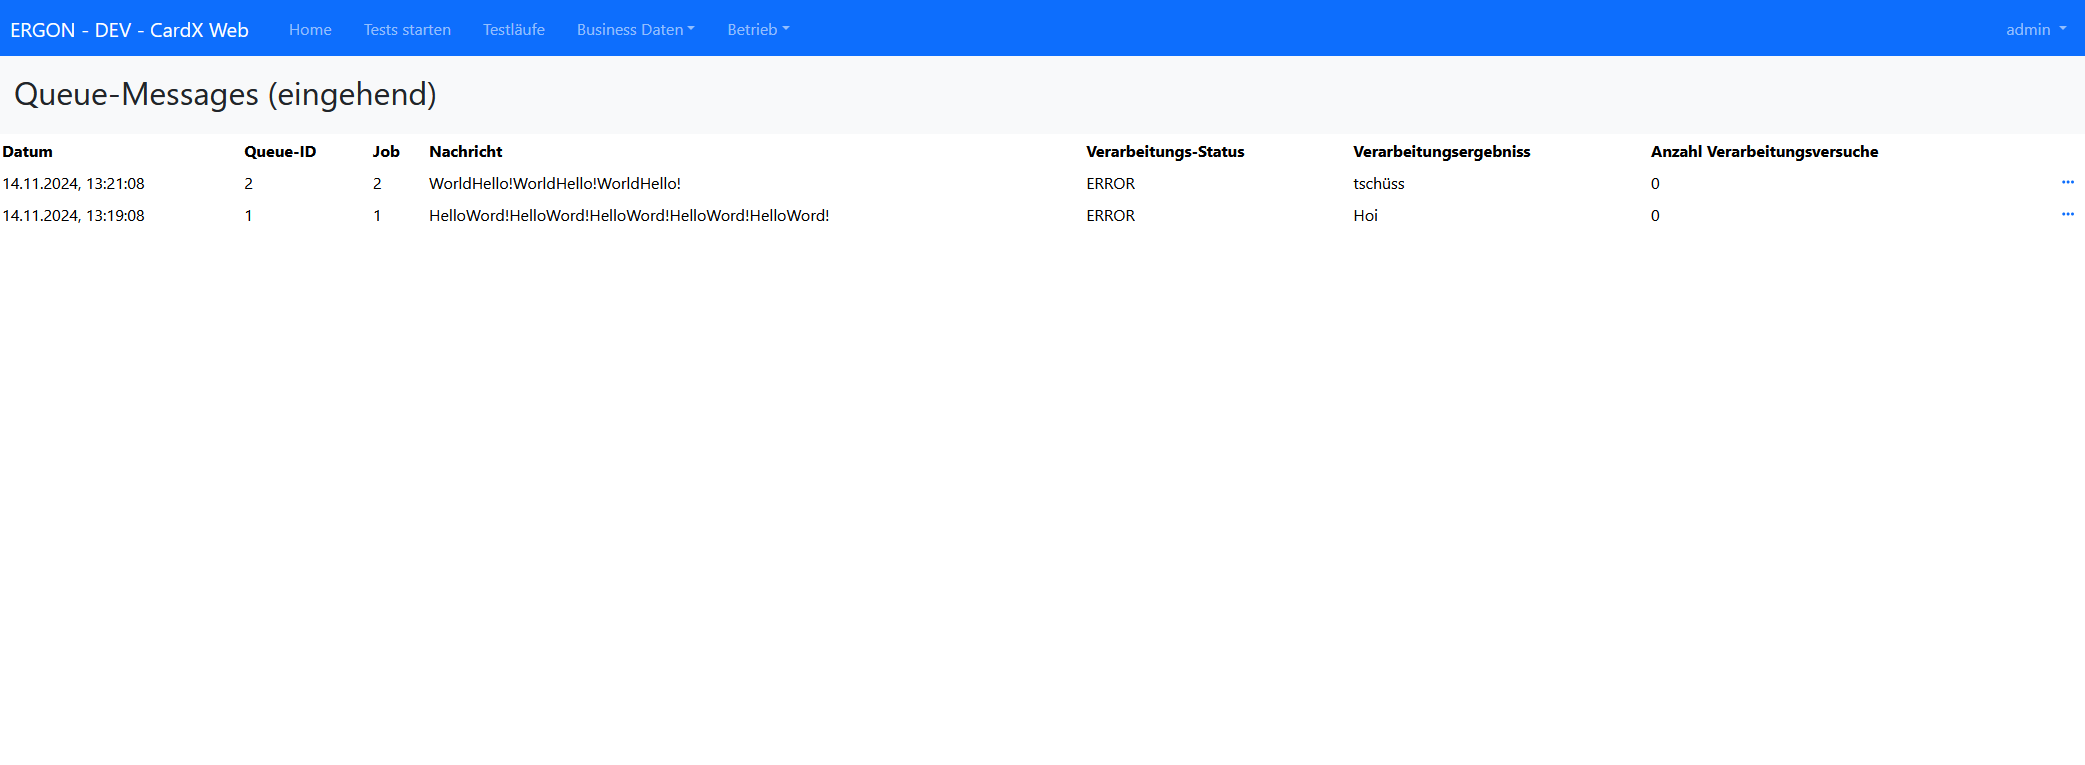
\includegraphics[width=1\textwidth]{ressourcen/4.2_Tabelle}
		\caption[Jenkins Codequalität]{Jenkins Codequalität}\label{ch:code-quality}
	\end{center}
\end{figure}

\subsection{Falscher Rückgabewert bei setMqInStatusToNew}
Die Funktion setMqInStatusToNew() hatte von den PMD-Warnungen aus einen falschen Rückgabewert (int). Diese Warnung tauchte auf wegen dem Namen. Da ein «set» im Namen vorhanden war, wurde vermutet, dass es einen Setter ist, was aber nicht der Fall war. Die Funktion wurde Darauf hin umbenennt zu executeNewProcessingAttempt().

\subsection{JUnit-Test Klassen müssen final sein}
Um die Sichtbarkeit der Testklassen einzuschränken müssen diese Package-private sein. Aus diesem Grund wurde die Sichtbarkeit von MqInIntegrationTest angepasst.

\subsection{LocalDateTime / -Millis.class}
Bei der Erstellung von den Mock-Daten in der Klasse MqInServiceMockImpl wurde der Datums-Typ LocalDateTime verwendet. Die Nutzung von diesem Typ wurde abgeraten und empfohlen den Typ LocalDateTimeMillis zu nehmen, da hier die Millisekunden auch angezeigt werden.

\subsection{MqInMocks}
Die Klasse MqInMocks hat einen privaten Konstruktor und sollte in diesem Fall selbst eine final Klasse sein.


\newpage
    \chapter{Auswerten}\label{ch:auswerten}
\newpage
    % Projekt Kapitel

    \printglossary[title=Glossar, toctitle=Glossar]

    \renewcommand*{\listfigurename}{Abbildungsverzeichnis}
\listoffigures
% Structure:
% \begin{figure}
% \captionsetup{textformat=empty, labelformat=empty} -> to hide the caption beneath the image
% \includegraphics[format]{resource}
% \caption[<caption> (<cite source>) | caption (Eigene Darstellung)]{<caption>}\label{fig:<label>}
% \end{figure}

    \printbibliography[
    heading=bibintoc,
    title=Quellenverzeichnis]


\end{document}
